\documentclass[11pt]{article}
\usepackage[utf8]{inputenc}
\usepackage[T1]{fontenc}
\usepackage[margin=1in]{geometry}
\usepackage{graphicx}
\usepackage{booktabs}
\usepackage{amsmath}
\usepackage{amssymb}
\usepackage{hyperref}
\usepackage{float}
\usepackage{subcaption}
\usepackage{xcolor}
\usepackage{longtable}
\usepackage{array}
\usepackage{placeins}
\usepackage{pdflscape}
\usepackage{adjustbox}
\usepackage{url}

\title{Reporte Mapper/TDA de exoplanetas PSCompPars imputados}
\author{}
\date{}

\begin{document}
\maketitle
\begin{abstract}


Este proyecto estudia la estructura de una población de exoplanetas confirmados del catálogo PSCompPars del NASA Exoplanet Archive mediante Mapper, una técnica de Topological Data Analysis aplicada sobre datos procesados e imputados. La motivación central no es producir una clasificación definitiva de planetas, sino explorar si las relaciones entre sus propiedades físicas, orbitales y térmicas generan regiones estructuradas que puedan ser interpretadas astrofísicamente. Al mismo tiempo, el proyecto reconoce que los datos de exoplanetas no son una muestra neutral: están afectados por valores faltantes, por decisiones de imputación y por sesgos observacionales asociados a los métodos de descubrimiento.

La pregunta que guía el análisis es si Mapper/TDA puede revelar regiones significativas en el espacio de propiedades de los exoplanetas, y hasta qué punto esas regiones reflejan señal física u orbital, sesgo observacional, dependencia de imputación o sensibilidad metodológica. Para responderla, se reconciliaron 21 grafos Mapper existentes, correspondientes a siete espacios de variables y tres lentes, todos construidos con la cubierta fija \texttt{cubes10\_overlap0p35}. Los espacios comparados incluyen variables físicas, orbitales, térmicas y combinadas. La interpretación principal se concentró en los grafos con lente \texttt{pca2}, mientras que los lentes \texttt{domain} y \texttt{density} se consideraron como capas de sensibilidad.

El grafo que emergió como candidato principal fue \texttt{orbital\_pca2\_cubes10\_overlap0p35}. Este Mapper contiene 124 nodos, 196 aristas y $\beta_1=96$, con una imputación media nodal de 0.011. Esta combinación lo vuelve especialmente interesante: muestra una estructura topológica rica, pero con baja dependencia de valores imputados. En contraste, el Mapper térmico también presenta complejidad, pero su imputación media nodal de 0.588 obliga a interpretarlo con mayor cautela.

Para evitar una lectura ingenua de la topología observada, se incorporó una auditoría de sesgo observacional. Las variables \texttt{discoverymethod}, \texttt{disc\_year} y \texttt{disc\_facility} no se usaron para construir los grafos, sino como metadata externa para evaluar si las regiones detectadas estaban asociadas con la forma en que los planetas fueron descubiertos. En el grafo orbital principal, la pureza observada ponderada por método fue 0.842, el NMI observado entre asignación nodal y método de descubrimiento fue 0.254, y la prueba nula por permutación produjo $p=0.001$. Esto sugiere que la estructura orbital contiene información relevante, pero también está significativamente asociada con sesgos de descubrimiento.

En conjunto, los resultados muestran que Mapper puede identificar regiones candidatas útiles para inspección científica, especialmente en el espacio orbital. Sin embargo, esas regiones no deben interpretarse como la topología real de los exoplanetas ni como una taxonomía final. La conclusión principal es mixta: hay evidencia de estructura física u orbital plausible, pero también una contribución medible del sesgo observacional y de la incertidumbre introducida por la imputación. Por ello, la aportación del proyecto es una lectura crítica de la topología observada, separando regiones con posible señal astrofísica de regiones observacionales, mixtas o débiles.


\end{abstract}

\newpage
\section{Resumen ejecutivo}
Este reporte está organizado alrededor de una idea central: no basta con construir grafos Mapper y observar que tienen estructura; también es necesario evaluar qué tipo de evidencia sostiene esa estructura. En este proyecto, Mapper se usa como una herramienta exploratoria para revelar regiones candidatas en el espacio de propiedades de exoplanetas. Después, esas regiones se auditan desde tres dimensiones: su dependencia de imputación, su posible interpretación física u orbital y su asociación con variables de sesgo observacional.

La lectura general del proyecto es que la estructura más informativa aparece en el espacio orbital. Sin embargo, esa estructura no puede tomarse directamente como una señal astrofísica pura, porque la auditoría por método de descubrimiento muestra una asociación estadísticamente significativa entre la topología del grafo y la forma en que los planetas fueron detectados. Por eso, el resultado más importante no es una clasificación cerrada de exoplanetas, sino una clasificación crítica de las regiones observadas: algunas parecen físicamente interpretables, otras parecen dominadas por sesgo observacional, algunas son mixtas y otras deben considerarse débiles por su dependencia de imputación o falta de evidencia suficiente.

\begin{table}[H]
\centering
\small
\begin{tabular}{p{0.43\textwidth}p{0.43\textwidth}}
\toprule
\textbf{Elemento evaluado} & \textbf{Resultado principal} \\
\midrule
Mappers reconciliados & 21 grafos completos \\
Diseño de comparación & 7 espacios de variables $\times$ 3 lentes \\
Cubierta usada & \texttt{cubes10\_overlap0p35} \\
Capa principal de interpretación & \texttt{pca2} \\
Grafo candidato principal & \texttt{orbital\_pca2\_cubes10\_overlap0p35} \\
Nodos del grafo orbital & 124 \\
Aristas del grafo orbital & 196 \\
Ciclos del grafo orbital & $\beta_1=96$ \\
Imputación media nodal orbital & 0.011 \\
Imputación media nodal térmica & 0.588 \\
Pureza observada por método en orbital & 0.842 \\
NMI entre nodo y \texttt{discoverymethod} & 0.254 \\
$p$ empírico por permutación & 0.001 \\
Lectura principal & Señal orbital informativa con sesgo observacional significativo \\
\bottomrule
\end{tabular}
\caption{Resumen ejecutivo de los hallazgos medibles principales del proyecto.}
\label{tab:executive_summary}
\end{table}

La Tabla~\ref{tab:executive_summary} resume la lógica de evidencia del proyecto. El Mapper orbital es el resultado más prometedor porque combina alta complejidad topológica con baja imputación. En cambio, el Mapper térmico muestra que una estructura compleja no necesariamente es más confiable si depende fuertemente de valores imputados. Esta comparación es importante porque obliga a distinguir entre una estructura visualmente rica y una estructura científicamente defendible.

La auditoría de sesgo observacional refuerza esta cautela. El hecho de que el grafo orbital tenga una asociación significativa con \texttt{discoverymethod} indica que parte de la topología observada puede estar relacionada con el proceso de recolección del catálogo. Esto no invalida el resultado orbital, pero sí cambia su interpretación: el grafo no debe leerse como una clasificación directa de arquitecturas planetarias, sino como una estructura donde se mezclan señal orbital, sesgo de descubrimiento y efectos del preprocesamiento.

En consecuencia, el reporte adopta una postura conservadora. Las regiones de Mapper se interpretan como candidatas para inspección astrofísica, no como clases finales. Una región será más confiable si combina baja imputación, coherencia física u orbital y baja asociación con método de descubrimiento. Una región será más sospechosa si está dominada por un método, una facilidad de descubrimiento o una época específica. Esta distinción permite que el análisis sea más fuerte: no solo muestra que hay estructura, sino que evalúa qué tan interpretable es esa estructura.


\newpage
\section{Introduccion y pregunta de investigacion}
El estudio de exoplanetas plantea un problema de estructura: no siempre esperamos encontrar grupos simples, separados y perfectamente definidos. Las propiedades planetarias cambian de forma continua. Un planeta puede ser pequeño pero muy irradiado, masivo pero lejano, denso pero con una órbita particular, o pertenecer a una región del catálogo que está sobrerrepresentada por un método de descubrimiento específico. Por eso, antes de asumir clases planetarias rígidas, resulta útil preguntarse si el catálogo contiene regiones conectadas, transiciones, ramas o ciclos que puedan ser inspeccionados desde una perspectiva astrofísica.

En este proyecto usamos Mapper, una técnica de Topological Data Analysis, para construir grafos exploratorios a partir de distintas selecciones de variables de exoplanetas. A diferencia de un clustering tradicional, Mapper no fuerza una partición única del catálogo. En lugar de asignar cada planeta a una sola clase, construye un grafo de regiones locales que pueden solaparse y conectarse entre sí. Esta propiedad es importante para este problema, porque muchas poblaciones planetarias no necesariamente aparecen como grupos compactos, sino como continuos o transiciones entre regímenes físicos, orbitales y térmicos.

La pregunta de investigación que guía el reporte es la siguiente:

\begin{quote}
¿Pueden los grafos Mapper construidos sobre variables físicas, orbitales, térmicas y combinadas de exoplanetas revelar regiones candidatas para inspección científica, y en qué medida esas regiones pueden confundirse con sesgo observacional, dependencia de imputación o sensibilidad metodológica?
\end{quote}

La lectura del proyecto es deliberadamente cautelosa. Mapper no se interpreta aquí como una prueba definitiva de estructura física ni como una taxonomía final de exoplanetas. En este trabajo, una ``estructura'' significa una organización medible dentro del grafo: número de nodos, aristas, componentes, ciclos, regiones con coherencia física u orbital, regiones dominadas por un método de descubrimiento, o regiones con alta o baja dependencia de imputación. En otras palabras, el grafo se entiende como un resumen exploratorio de vecindades inducidas por una matriz de datos procesada y completada, no como la topología real de la población planetaria.

El análisis compara varias maneras de mirar el mismo catálogo. El espacio físico aproxima qué tipo de planeta es un objeto mediante variables como radio, masa y densidad. El espacio orbital describe dónde vive y cómo se organiza su órbita mediante periodo orbital y semieje mayor. El espacio térmico aproxima el ambiente energético mediante insolación y temperatura de equilibrio. Finalmente, los espacios conjuntos permiten observar cómo se combinan estas descripciones. Esta separación es central porque evita mezclar todas las variables desde el inicio y permite preguntar qué tipo de estructura produce cada perspectiva.

A partir de esta pregunta general, el reporte evalúa cuatro hipótesis de trabajo. Primero, una hipótesis física u orbital: algunos espacios de variables, especialmente el orbital, podrían producir grafos con estructura topológica rica y regiones interpretables. Segundo, una hipótesis de imputación: las estructuras que dependen fuertemente de variables imputadas deben considerarse menos confiables. Tercero, una hipótesis de sesgo observacional: algunas regiones Mapper podrían estar enriquecidas por \texttt{discoverymethod}, \texttt{disc\_year} o \texttt{disc\_facility}, lo que indicaría que parte de la topología refleja el proceso de descubrimiento más que una diferencia física intrínseca. Cuarto, una hipótesis mixta: la estructura observada probablemente no será puramente física ni puramente observacional, sino una combinación de señal astrofísica, sesgo de detección y decisiones metodológicas.

Esta distinción es importante porque una región del grafo puede parecer científicamente interesante por varias razones distintas. Puede ser compatible con una señal astrofísica si muestra coherencia en radio, masa, densidad, periodo orbital, insolación o temperatura. Puede ser metodológicamente confiable si aparece con baja imputación y no depende de una sola construcción del lente. Pero también puede ser observacionalmente sospechosa si está dominada por un solo método de descubrimiento, por una facilidad específica o por una época de observación. Por eso, en lugar de concluir directamente que una rama o componente representa una familia planetaria, el análisis pregunta qué tipo de evidencia sostiene esa región.

El objetivo del reporte, entonces, no es decir simplemente si ``hay clases'' o ``no hay clases''. El objetivo es descomponer la topología observada en varias fuentes de evidencia:

\[
\text{topología observada}
=
\text{señal física/orbital}
+
\text{sesgo observacional}
+
\text{efecto de imputación}
+
\text{sensibilidad metodológica}.
\]

Bajo esta formulación, una conclusión fuerte no sería afirmar que Mapper descubre una clasificación definitiva de exoplanetas, sino identificar qué regiones son candidatas a interpretación física, cuáles parecen dominadas por sesgo observacional, cuáles mezclan ambos efectos y cuáles deben considerarse débiles. Esta lectura permite aprovechar la riqueza del catálogo sin ignorar las limitaciones de los datos con los que fue construido.
\section{Contexto astrofisico y variables}
El análisis se construyó a partir de una separación astrofísica de las variables. En lugar de usar todas las columnas disponibles del catálogo al mismo tiempo, las variables se organizaron en espacios con significado físico: propiedades corporales del planeta, propiedades orbitales, propiedades térmicas y combinaciones entre ellas. Esta decisión es importante porque Mapper es sensible a la escala, a la redundancia entre variables y a los valores faltantes. Por ello, cada espacio de variables responde una pregunta distinta sobre la población de exoplanetas.

Las variables físicas describen qué tipo de objeto planetario se está observando. En este bloque se usan principalmente \texttt{pl\_rade}, \texttt{pl\_bmasse} y, en algunos espacios, \texttt{pl\_dens}. El radio permite distinguir planetas pequeños, sub-Neptunos, Neptunos y gigantes; la masa aporta información sobre escala gravitacional y composición posible; y la densidad resume la relación entre masa y volumen. En conjunto, estas variables aproximan la naturaleza física del planeta: si es compatible con un cuerpo rocoso, un planeta con envoltura gaseosa o un gigante gaseoso.

Las variables orbitales describen el entorno dinámico del planeta, es decir, dónde vive dentro de su sistema. En los artefactos reconciliados de este proyecto, el espacio orbital usa \texttt{pl\_orbper} y \texttt{pl\_orbsmax}. El periodo orbital indica cuánto tarda el planeta en completar una órbita, mientras que el semieje mayor aproxima su distancia media a la estrella. Estas variables permiten separar, por ejemplo, planetas de periodo corto y órbitas cercanas de planetas con órbitas más amplias o periodos largos.

Las variables térmicas describen el ambiente energético del planeta. El espacio \texttt{thermal} usa \texttt{pl\_insol} y \texttt{pl\_eqt}. La insolación mide cuánta radiación recibe el planeta en comparación con la Tierra, mientras que la temperatura de equilibrio estima la temperatura esperada bajo un modelo simplificado de balance radiativo. Estas variables son útiles para distinguir planetas muy calientes, calientes, templados o fríos. Sin embargo, en este proyecto el bloque térmico debe interpretarse con cautela, porque mostró una dependencia mucho mayor de imputación que el bloque orbital.

Los espacios de variables existentes en los artefactos reconciliados son:
\[
\texttt{joint},\quad
\texttt{joint\_no\_density},\quad
\texttt{orb\_thermal},\quad
\texttt{orbital},\quad
\texttt{phys\_density},\quad
\texttt{phys\_min},\quad
\texttt{thermal}.
\]
Estos espacios permiten comparar distintas maneras de mirar el mismo catálogo. \texttt{phys\_min} usa las variables físicas principales sin densidad; \texttt{phys\_density} agrega densidad como control físico; \texttt{orbital} se concentra en la escala orbital; \texttt{thermal} resume el ambiente energético; \texttt{orb\_thermal} combina órbita y energía recibida; y los espacios \texttt{joint} y \texttt{joint\_no\_density} permiten evaluar la estructura conjunta con y sin densidad.

\begin{table}[H]
\centering
\small
\begin{tabular}{p{0.25\textwidth}p{0.35\textwidth}p{0.30\textwidth}}
\toprule
\textbf{Espacio} & \textbf{Variables} & \textbf{Interpretación principal} \\
\midrule
\texttt{phys\_min} & \texttt{pl\_rade}, \texttt{pl\_bmasse} & Tamaño y masa del planeta \\
\texttt{phys\_density} & \texttt{pl\_rade}, \texttt{pl\_bmasse}, \texttt{pl\_dens} & Propiedades físicas incluyendo densidad \\
\texttt{orbital} & \texttt{pl\_orbper}, \texttt{pl\_orbsmax} & Escala orbital: periodo y distancia media \\
\texttt{thermal} & \texttt{pl\_insol}, \texttt{pl\_eqt} & Ambiente energético del planeta \\
\texttt{orb\_thermal} & \texttt{pl\_orbper}, \texttt{pl\_orbsmax}, \texttt{pl\_insol}, \texttt{pl\_eqt} & Relación entre órbita y ambiente térmico \\
\texttt{joint\_no\_density} & Físicas, orbitales y térmicas sin \texttt{pl\_dens} & Estructura conjunta sin densidad derivada \\
\texttt{joint} & Físicas, orbitales y térmicas con \texttt{pl\_dens} & Estructura conjunta incluyendo densidad \\
\bottomrule
\end{tabular}
\caption{Espacios de variables usados para construir los grafos Mapper reconciliados.}
\label{tab:feature_spaces_context}
\end{table}

Un punto importante es que el espacio orbital seleccionado no incluye excentricidad. El grafo \texttt{orbital\_pca2\_cubes10\_overlap0p35} fue construido con las variables registradas en su JSON de configuración: \texttt{pl\_orbper} y \texttt{pl\_orbsmax}. Por lo tanto, en los artefactos reconciliados, \texttt{pl\_orbeccen} no forma parte de las coordenadas del Mapper orbital actual. Esto no significa que la excentricidad sea irrelevante; al contrario, físicamente describe la forma de la órbita y puede distinguir órbitas circulares de órbitas altamente elípticas. La decisión aquí es metodológica: como el objetivo del reporte es auditar e interpretar los grafos ya generados, incluir excentricidad requeriría construir un nuevo espacio orbital y correr nuevos Mappers. Por ello, \texttt{pl\_orbeccen} se considera una extensión futura de sensibilidad orbital, no una variable activa de la interpretación principal.

También es necesario tratar la densidad con cuidado. La densidad planetaria es una variable físicamente útil porque relaciona masa y radio, y puede ayudar a distinguir cuerpos rocosos de planetas gaseosos o de baja densidad. Sin embargo, cuando \texttt{pl\_dens} se usa junto con \texttt{pl\_bmasse} y \texttt{pl\_rade}, no debe interpretarse como evidencia completamente independiente. En la auditoría de derivaciones, 6199 valores de \texttt{pl\_dens} fueron derivados a partir de masa y radio; antes de la derivación había 6273 valores faltantes y después quedaron 74. Esta dependencia algebraica justifica comparar explícitamente espacios con y sin densidad. Por eso \texttt{phys\_density} y \texttt{joint} funcionan como controles de sensibilidad, mientras que \texttt{phys\_min} y \texttt{joint\_no\_density} permiten observar la estructura sin incorporar una variable derivada.

Además de las variables usadas como coordenadas de Mapper, el proyecto conserva variables de auditoría. \texttt{discoverymethod}, \texttt{disc\_year} y \texttt{disc\_facility} no describen al planeta como objeto físico, sino el proceso mediante el cual fue descubierto. Por esa razón no se usan como variables de entrada del Mapper. Incluirlas directamente en la geometría podría producir grafos que agrupen planetas por su historia observacional en vez de por sus propiedades físicas u orbitales. En cambio, se usan después como metadata externa para preguntar si las regiones del grafo están enriquecidas por método, época o instalación de descubrimiento.

Esta distinción es clave porque los métodos de detección no observan de manera uniforme toda la población planetaria. El método de tránsito favorece planetas con periodos cortos y radios grandes, porque producen caídas de brillo más frecuentes y detectables. La velocidad radial favorece planetas masivos, especialmente si inducen variaciones medibles en la estrella. La imagen directa favorece objetos jóvenes, masivos, luminosos y separados de su estrella. Por lo tanto, una región Mapper dominada por un solo método de descubrimiento puede reflejar tanto una estructura física real como una huella del proceso de observación.

Finalmente, las etiquetas interpretativas usadas en el análisis, como \texttt{radius\_class}, \texttt{density\_class}, \texttt{orbit\_class}, \texttt{thermal\_class} o \texttt{candidate\_population}, deben leerse como apoyos heurísticos y no como una taxonomía definitiva. Su función es ayudar a describir qué tipo de planetas aparecen en cada nodo o componente del grafo. Una región será más convincente si combina coherencia física u orbital, baja imputación y baja asociación con \texttt{discoverymethod}. Una región será más sospechosa si está dominada por un método de descubrimiento, una facilidad específica o una alta proporción de valores imputados.
\section{Datos, imputacion y cantidades derivadas}
El análisis parte de la tabla \texttt{PSCompPars} del NASA Exoplanet Archive, específicamente del archivo compacto \texttt{data/PSCompPars\_2026.04.25\_17.36.36.csv}. Esta versión contiene 6273 exoplanetas y 84 columnas. A partir de esta tabla se construyó una versión procesada e imputada del catálogo para poder alimentar los espacios de variables usados por Mapper.

La imputación fue necesaria porque Mapper requiere una matriz numérica completa para construir los grafos. Si se trabajara únicamente con casos completos, se perdería una parte importante del catálogo y algunos espacios de análisis quedarían severamente reducidos. El problema es especialmente visible en las variables térmicas, como \texttt{pl\_insol} y \texttt{pl\_eqt}, y en variables que no estaban completas en la tabla compacta, como \texttt{pl\_dens}. Por esta razón, el pipeline no solo imputó valores faltantes, sino que también conservó trazabilidad sobre qué valores fueron observados, derivados físicamente o imputados estadísticamente.

\subsection*{Disponibilidad inicial de variables}

Las variables principales usadas para Mapper presentaban distintos niveles de faltantes antes de la imputación o derivación. La Tabla~\ref{tab:raw_missing_values} resume la disponibilidad inicial de las variables principales.

\begin{table}[H]
\centering
\small
\begin{tabular}{lrrp{0.38\textwidth}}
\toprule
\textbf{Variable} & \textbf{Faltantes crudos} & \textbf{Total} & \textbf{Comentario} \\
\midrule
\texttt{pl\_rade} & 50 & 6273 & Radio planetario; variable física principal. \\
\texttt{pl\_bmasse} & 31 & 6273 & Masa planetaria; variable física principal. \\
\texttt{pl\_dens} & 6273 & 6273 & No venía completa en la tabla compacta; se derivó para la mayoría de planetas. \\
\texttt{pl\_orbper} & 339 & 6273 & Periodo orbital; variable orbital principal. \\
\texttt{pl\_orbsmax} & 428 & 6273 & Semieje mayor; se derivó cuando fue posible. \\
\texttt{pl\_insol} & 1876 & 6273 & Insolación; variable térmica con alta incompletitud. \\
\texttt{pl\_eqt} & 1600 & 6273 & Temperatura de equilibrio; variable térmica con alta incompletitud. \\
\bottomrule
\end{tabular}
\caption{Valores faltantes crudos en las variables principales antes de imputación o derivación física.}
\label{tab:raw_missing_values}
\end{table}

Esta tabla muestra que no todas las variables tienen el mismo nivel de confiabilidad inicial. Las variables físicas básicas, como radio y masa, tienen pocos faltantes. En cambio, las variables térmicas tienen una proporción mucho mayor de valores ausentes. Esto anticipa una diferencia importante en la interpretación posterior: un grafo puede ser topológicamente complejo, pero si esa complejidad depende de variables altamente imputadas, debe interpretarse con cautela.

\subsection*{Derivaciones físicas}

Antes de aplicar imputación estadística, el pipeline intentó completar algunas variables mediante relaciones físicas conocidas. Esta diferencia es importante: una variable derivada no es una observación directa, pero tampoco es una imputación puramente estadística. Es un valor calculado a partir de otras mediciones disponibles.

La primera derivación fue la densidad planetaria, calculada a partir de masa y radio:

\[
\texttt{pl\_dens}
=
5.514
\times
\frac{\texttt{pl\_bmasse}}{\texttt{pl\_rade}^{3}}.
\]

El factor 5.514 corresponde a la densidad media de la Tierra en g/cm$^3$, de modo que la fórmula convierte la relación masa-radio en una densidad planetaria aproximada. En la tabla compacta, \texttt{pl\_dens} tenía 6273 valores faltantes antes de la derivación. El pipeline derivó 6199 valores y dejó 74 faltantes después de esta etapa.

La segunda derivación fue el semieje mayor, usando una relación tipo Kepler a partir del periodo orbital y la masa estelar:

\[
\texttt{pl\_orbsmax}
=
\left(
\texttt{st\_mass}
\times
\left(
\frac{\texttt{pl\_orbper}}{365.25}
\right)^2
\right)^{1/3}.
\]

Antes de esta derivación, \texttt{pl\_orbsmax} tenía 428 valores faltantes. El pipeline derivó 420 valores y dejó 8 faltantes después de la etapa de derivación.

\begin{table}[H]
\centering
\small
\begin{tabular}{lrrrp{0.28\textwidth}}
\toprule
\textbf{Variable derivada} & \textbf{Faltantes antes} & \textbf{Derivados} & \textbf{Faltantes después} & \textbf{Fuente de derivación} \\
\midrule
\texttt{pl\_dens} & 6273 & 6199 & 74 & Masa y radio planetario. \\
\texttt{pl\_orbsmax} & 428 & 420 & 8 & Periodo orbital y masa estelar. \\
\bottomrule
\end{tabular}
\caption{Variables completadas mediante derivaciones físicas antes de la imputación estadística.}
\label{tab:physical_derivations}
\end{table}

Estas derivaciones tienen consecuencias directas para la interpretación. En particular, \texttt{pl\_dens} debe tratarse como una variable de control y no como evidencia completamente independiente cuando se usa junto con \texttt{pl\_rade} y \texttt{pl\_bmasse}. Como la densidad se calcula a partir de masa y radio, puede reforzar patrones ya contenidos algebraicamente en esas variables. Por eso el reporte compara explícitamente espacios con densidad y sin densidad, como \texttt{phys\_density} frente a \texttt{phys\_min}, y \texttt{joint} frente a \texttt{joint\_no\_density}.

\subsection*{Imputación estadística}

Después de las derivaciones físicas, el pipeline aplicó imputación estadística para completar la matriz de variables usada por Mapper. Se compararon tres métodos: \texttt{median}, \texttt{knn} e \texttt{iterative}. El método principal seleccionado fue \texttt{iterative}, porque obtuvo el mejor ranking promedio en las métricas de validación, considerando MAE y RMSE. En esta lectura, \texttt{median} funciona como una línea base robusta, \texttt{knn} como alternativa intermedia, e \texttt{iterative} como el método principal para los resultados visualizados e interpretados.

Es importante separar conceptualmente las variables derivadas de las imputadas. Una variable derivada se calcula usando una relación física y otras mediciones disponibles. Una variable imputada se estima estadísticamente a partir de patrones del dataset. Ambas introducen incertidumbre, pero no la misma clase de incertidumbre. Por eso el análisis conserva banderas de trazabilidad y no trata la matriz final como si todos sus valores tuvieran el mismo origen.

\begin{quote}
\textbf{Distinción metodológica.} En este reporte, ``derivado'' significa calculado mediante una relación física a partir de otras variables observadas; ``imputado'' significa estimado estadísticamente para completar valores faltantes. Ambos casos se auditan, pero no se interpretan como equivalentes.
\end{quote}

\subsection*{Trazabilidad de imputación y fuentes}

La imputación no se trató como un paso invisible del pipeline. Por planeta, la tabla completa imputada conservó columnas de trazabilidad que permiten identificar si un valor fue observado, faltante, derivado físicamente o imputado. Entre estas columnas se encuentran:

\[
\texttt{*\_was\_missing},\quad
\texttt{*\_was\_observed},\quad
\texttt{*\_was\_physically\_derived},\quad
\texttt{*\_was\_imputed},\quad
\texttt{*\_source},\quad
\texttt{imputation\_method}.
\]

Estas columnas aparecen especialmente en \texttt{reports/imputation/PSCompPars\_imputed\_iterative.csv}. Después, al construir los grafos Mapper, esta trazabilidad se agregó por nodo. Esto permitió calcular métricas de confianza como:

\[
\texttt{mean\_imputation\_fraction},\quad
\texttt{median\_imputation\_fraction},\quad
\texttt{observed\_fraction},\quad
\texttt{physically\_derived\_fraction},\quad
\texttt{imputed\_fraction},\quad
\texttt{frac\_any\_imputed}.
\]

Estas métricas aparecen en tablas como \texttt{node\_physical\_interpretation.csv} y \texttt{mapper\_node\_source\_audit.csv}. Su función es permitir que cada nodo o región del Mapper se evalúe no solo por su posición topológica, sino también por la calidad de la información que lo sostiene.

\subsection*{Confianza por espacio de variables}

La auditoría de imputación muestra que los espacios de variables no tienen el mismo nivel de confiabilidad. La Tabla~\ref{tab:imputation_by_space} resume las métricas principales para los grafos seleccionados.

\begin{table}[H]
\centering
\small
\begin{tabular}{lrrp{0.36\textwidth}}
\toprule
\textbf{Grafo seleccionado} & \textbf{Imputación media nodal} & \textbf{Riesgo} & \textbf{Interpretación} \\
\midrule
\texttt{phys\_min\_pca2\_cubes10\_overlap0p35} & 0.017 & Bajo & Espacio físico básico con poca dependencia de imputación. \\
\texttt{phys\_density\_pca2\_cubes10\_overlap0p35} & 0.002 & Bajo/moderado & Baja imputación, pero densidad frecuentemente derivada. \\
\texttt{orbital\_pca2\_cubes10\_overlap0p35} & 0.011 & Bajo & Espacio orbital confiable por imputación y candidato principal de inspección. \\
\texttt{joint\_no\_density\_pca2\_cubes10\_overlap0p35} & 0.176 & Moderado & Incluye variables térmicas, por lo que aumenta la dependencia de imputación. \\
\texttt{joint\_pca2\_cubes10\_overlap0p35} & 0.152 & Moderado & Espacio conjunto con densidad; combina riesgo térmico y redundancia de densidad. \\
\texttt{thermal\_pca2\_cubes10\_overlap0p35} & 0.588 & Alto & Estructura térmica con fuerte dependencia de imputación. \\
\bottomrule
\end{tabular}
\caption{Dependencia de imputación en los grafos seleccionados.}
\label{tab:imputation_by_space}
\end{table}

La lectura principal es que los espacios físico y orbital tienen baja dependencia de imputación, mientras que el espacio térmico tiene un riesgo mucho mayor. En particular, \texttt{thermal\_pca2\_cubes10\_overlap0p35} tiene una imputación media nodal de 0.588 y una fracción de nodos con alta imputación de 0.719. Esto no significa que el grafo térmico no contenga información, pero sí que cualquier interpretación astrofísica derivada de ese espacio debe ser más conservadora.

Los espacios conjuntos, \texttt{joint\_no\_density} y \texttt{joint}, tienen riesgo moderado porque incorporan variables térmicas como \texttt{pl\_insol} y \texttt{pl\_eqt}, que son precisamente las variables más incompletas. Por lo tanto, los espacios conjuntos son útiles para comparar perspectivas, pero no necesariamente producen evidencia más fuerte que los espacios simples. En este proyecto, la interpretación más confiable surge cuando una región combina baja imputación, coherencia física u orbital y baja asociación con sesgos de descubrimiento.

\subsection*{Implicaciones para la interpretación de Mapper}

La consecuencia metodológica de esta sección es que la imputación se usa como criterio de confianza. Un nodo Mapper no se interpreta únicamente por su posición en el grafo o por las variables promedio de sus planetas, sino también por el origen de sus datos. Una región con baja imputación puede sostener mejor una interpretación física u orbital. En cambio, una región con alta imputación, aunque sea topológicamente compleja, debe considerarse débil o cautelosa.

Esta distinción explica por qué el grafo orbital se vuelve especialmente importante en el reporte: combina baja imputación media nodal con alta complejidad topológica. En contraste, el grafo térmico puede mostrar estructura, pero su dependencia de imputación reduce la fuerza de cualquier conclusión física directa. Así, la imputación no aparece solo como un paso técnico previo, sino como una parte central de la evaluación científica de las regiones Mapper.
\section{Metodologia Mapper}
Sea $X = \{x_1, \ldots, x_n\} \subset \mathbb{R}^p$. Sea $f: X \to \mathbb{R}^d$ un lens. Para cada cubierta del espacio de lentes se clusteriza la preimagen y se construye un grafo por interseccion de clusters locales. Usamos $\beta_1 = E - V + C$ con $C=\beta_0$. Las etiquetas fisicas de planetas son resumentes heuristicas, no taxonomias confirmadas.

\section{Reconciliacion de salidas y reproducibilidad}
Antes de interpretar los grafos Mapper, fue necesario reconciliar las salidas existentes del repositorio. El problema principal era que los artefactos individuales guardados en \texttt{outputs/mapper/} no coincidían completamente con las tablas agregadas activas usadas por el reporte. En particular, existían archivos para 21 grafos Mapper, pero las tablas agregadas principales resumían únicamente siete grafos con lente \texttt{pca2}. Es decir, había más resultados generados que resultados integrados en las tablas de interpretación.

Esta diferencia es importante porque el reporte no debe basarse en una lectura ambigua de los archivos disponibles. Si un grafo existe como artefacto individual, pero no aparece en las tablas agregadas, no queda claro si forma parte de la interpretación activa o si es un resultado anterior no sincronizado. Por eso se implementó una etapa de reconciliación para distinguir entre artefactos existentes, tablas activas y resultados efectivamente usados para la interpretación científica.

La reconciliación encontró 21 archivos de grafos en formato JSON, 21 archivos de nodos en formato CSV, 21 archivos de aristas en formato CSV y 21 archivos de configuración en formato JSON. Además, se verificó que cada grafo tuviera su archivo correspondiente de nodos, aristas y configuración. Por lo tanto, los artefactos existentes forman 21 conjuntos completos:

\[
\text{graph} + \text{nodes} + \text{edges} + \text{config}.
\]

Estos 21 conjuntos corresponden a la combinación de siete espacios de variables y tres lentes:

\[
7 \text{ espacios de variables} \times 3 \text{ lentes} = 21 \text{ grafos Mapper}.
\]

\begin{table}[H]
\centering
\small
\begin{tabular}{lr}
\toprule
\textbf{Tipo de artefacto} & \textbf{Cantidad encontrada} \\
\midrule
Archivos de grafos JSON & 21 \\
Archivos de nodos CSV & 21 \\
Archivos de aristas CSV & 21 \\
Archivos de configuración JSON & 21 \\
Conjuntos completos graph--nodes--edges--config & 21 \\
Espacios de variables & 7 \\
Lentes & 3 \\
\bottomrule
\end{tabular}
\caption{Resumen de artefactos Mapper encontrados durante la reconciliación de salidas.}
\label{tab:output_reconciliation_counts}
\end{table}

La diferencia central está entre los artefactos existentes y las tablas agregadas activas. Los artefactos existentes son los archivos individuales producidos por las corridas Mapper, ubicados en carpetas como \texttt{outputs/mapper/graphs/}, \texttt{outputs/mapper/nodes/}, \texttt{outputs/mapper/edges/} y \texttt{outputs/mapper/config/}. En cambio, las tablas agregadas activas son resúmenes ya procesados, como métricas de grafos, comparación entre espacios, sensibilidad por lente y selección de grafos principales. La reconciliación mostró que estas tablas activas no estaban sincronizadas con todos los artefactos existentes.

En particular, las tablas agregadas originales estaban restringidas a la capa \texttt{pca2}. Esto sugiere que una etapa posterior del pipeline generó o sobrescribió las tablas principales enfocándose únicamente en los grafos \texttt{pca2}, que son los usados para la interpretación central. Sin embargo, los artefactos individuales conservaban también grafos construidos con las lentes \texttt{domain} y \texttt{density}. Por esta razón, el reporte distingue entre la capa activa de interpretación y las capas disponibles para sensibilidad metodológica.

Para resolver esta desalineación sin borrar ni modificar las tablas originales, se reconstruyeron nuevas tablas con el sufijo \texttt{\_all\_existing}. Estas tablas resumen todos los artefactos encontrados, no solamente los grafos \texttt{pca2}. Los archivos reconstruidos fueron:

\begin{itemize}
    \item \texttt{output\_manifest.csv}
    \item \texttt{output\_consistency\_warnings.md}
    \item \texttt{mapper\_graph\_metrics\_all\_existing.csv}
    \item \texttt{mapper\_lens\_sensitivity\_all\_existing.csv}
    \item \texttt{mapper\_space\_comparison\_all\_existing.csv}
\end{itemize}

El archivo \texttt{output\_manifest.csv} funciona como inventario de los artefactos existentes. Registra qué grafos tienen archivos correspondientes de nodos, aristas y configuración, y permite identificar qué artefactos aparecen o no en las tablas agregadas activas. Por su parte, \texttt{mapper\_graph\_metrics\_all\_existing.csv} reconstruye métricas topológicas para los 21 grafos disponibles, mientras que las tablas de sensibilidad por lente y comparación por espacio permiten revisar de forma más completa las salidas ya generadas.

Un resultado importante de esta reconciliación es que no hay evidencia de una grilla completa de hiperparámetros en \texttt{n\_cubes} y \texttt{overlap}. Aunque el código puede soportar múltiples combinaciones, los artefactos existentes corresponden a una sola configuración de cubierta:

\[
\texttt{n\_cubes}=10,\qquad \texttt{overlap}=0.35.
\]

En los nombres de los grafos esta configuración aparece como \texttt{cubes10\_overlap0p35}. Por lo tanto, el análisis no debe describirse como una búsqueda completa de hiperparámetros. La formulación correcta es que se compararon espacios de variables y lentes bajo una cubierta fija.

\begin{quote}
\textbf{Nota de alcance.} Este reporte no interpreta los resultados como una grilla completa de \texttt{n\_cubes} y \texttt{overlap}. Los artefactos reconciliados permiten comparar siete espacios de variables y tres lentes, pero todos bajo la misma cubierta \texttt{cubes10\_overlap0p35}.
\end{quote}

A partir de esta reconciliación, la capa activa de interpretación del reporte se define como el conjunto de grafos seleccionados con lente \texttt{pca2}, listados en \texttt{outputs/mapper/tables/main\_graph\_selection.csv}. Esta decisión no implica que los grafos \texttt{domain} y \texttt{density} sean irrelevantes. Más bien, estos se tratan como capas de sensibilidad metodológica: sirven para revisar si la estructura observada depende fuertemente del lente usado, pero no constituyen la base principal de las conclusiones.

En resumen, la reconciliación de salidas cumple tres funciones. Primero, confirma que existen 21 grafos Mapper completos. Segundo, aclara que las tablas activas originales estaban enfocadas en \texttt{pca2}. Tercero, delimita el alcance metodológico del reporte: la interpretación científica principal se basa en los grafos \texttt{pca2} seleccionados, mientras que los demás lentes se usan como evidencia complementaria de sensibilidad. Esta separación permite que las conclusiones sean reproducibles y evita sobreafirmar una búsqueda de hiperparámetros que no está materializada en los artefactos actuales.
\section{Resultados principales de Mapper}
A partir de los grafos Mapper reconciliados, la interpretación principal del reporte se concentró en seis grafos con lente \texttt{pca2}. Esta selección permite comparar espacios físicos, orbitales, térmicos y conjuntos bajo una misma configuración de cubierta, \texttt{cubes10\_overlap0p35}. Los grafos seleccionados no cumplen todos la misma función: algunos se usan como resultados primarios, otros como controles metodológicos y uno como caso cauteloso por su alta dependencia de imputación.

Los grafos primarios son aquellos que permiten interpretar directamente una dimensión central del problema: la estructura física mínima, la estructura orbital y la estructura conjunta sin densidad. Los grafos de control permiten evaluar el efecto de agregar \texttt{pl\_dens}, una variable físicamente útil pero algebraicamente dependiente de masa y radio en gran parte del catálogo. El grafo térmico se conserva como resultado de interés, pero se etiqueta como \textit{cautionary} porque su estructura depende fuertemente de variables imputadas.

\begin{table}[H]
\centering
\small
\begin{tabular}{p{0.48\textwidth}p{0.18\textwidth}p{0.24\textwidth}}
\toprule
\textbf{Grafo seleccionado} & \textbf{Rol} & \textbf{Lectura principal} \\
\midrule
\texttt{phys\_min\_pca2\_cubes10\_overlap0p35} & Primario & Estructura física mínima usando radio y masa. \\
\texttt{phys\_density\_pca2\_cubes10\_overlap0p35} & Control & Efecto de agregar densidad al espacio físico. \\
\texttt{orbital\_pca2\_cubes10\_overlap0p35} & Primario & Estructura orbital principal. \\
\texttt{joint\_no\_density\_pca2\_cubes10\_overlap0p35} & Primario & Estructura conjunta sin densidad derivada. \\
\texttt{joint\_pca2\_cubes10\_overlap0p35} & Control & Efecto de agregar densidad al espacio conjunto. \\
\texttt{thermal\_pca2\_cubes10\_overlap0p35} & Cautionary & Estructura térmica con alta dependencia de imputación. \\
\bottomrule
\end{tabular}
\caption{Grafos \texttt{pca2} seleccionados para la interpretación principal del reporte.}
\label{tab:selected_pca2_graphs}
\end{table}

Entre los grafos seleccionados, el resultado estructuralmente más complejo es \texttt{orbital\_pca2\_cubes10\_overlap0p35}. Este grafo tiene 124 nodos, 196 aristas y $\beta_1=96$, el valor más alto de ciclos entre los grafos seleccionados. Esta combinación lo convierte en el principal candidato para inspección científica, porque presenta una topología rica sin depender fuertemente de imputación.

La importancia del grafo orbital no debe entenderse como prueba definitiva de una estructura física real. Más bien, indica que el espacio definido por \texttt{pl\_orbper} y \texttt{pl\_orbsmax} produce un grafo con alta conectividad y múltiples ciclos. Esto sugiere que la arquitectura orbital del catálogo contiene regiones y transiciones interesantes, pero su interpretación final requiere revisar imputación, sesgo observacional y coherencia astrofísica.

\begin{table}[H]
\centering
\small
\begin{tabular}{p{0.43\textwidth}rrrr}
\toprule
\textbf{Grafo} & \textbf{Nodos} & \textbf{Aristas} & $\boldsymbol{\beta_1}$ & \textbf{Imputación media} \\
\midrule
\texttt{phys\_min\_pca2\_cubes10\_overlap0p35} & 66 & 105 & 54 & 0.017 \\
\texttt{phys\_density\_pca2\_cubes10\_overlap0p35} & 67 & 102 & 52 & 0.002 \\
\texttt{orbital\_pca2\_cubes10\_overlap0p35} & 124 & 196 & 96 & 0.011 \\
\texttt{joint\_no\_density\_pca2\_cubes10\_overlap0p35} & 62 & 134 & 81 & 0.176 \\
\texttt{joint\_pca2\_cubes10\_overlap0p35} & 56 & 126 & 77 & 0.152 \\
\texttt{thermal\_pca2\_cubes10\_overlap0p35} & 121 & 150 & 67 & 0.588 \\
\bottomrule
\end{tabular}
\caption{Métricas principales de los grafos seleccionados.}
\label{tab:selected_graph_metrics}
\end{table}

La Tabla~\ref{tab:selected_graph_metrics} muestra que la complejidad topológica por sí sola no basta para seleccionar un grafo como evidencia fuerte. El grafo térmico, por ejemplo, también presenta una estructura considerable, con 121 nodos, 150 aristas y $\beta_1=67$. Sin embargo, su imputación media nodal es 0.588, mucho mayor que la del grafo orbital. Esto significa que la estructura térmica puede ser informativa, pero no debe interpretarse con la misma confianza que una estructura sostenida por variables con baja imputación.

En contraste, el grafo orbital combina dos propiedades deseables: alta complejidad y baja imputación. Su imputación media nodal es 0.011, lo que lo vuelve más confiable que el grafo térmico para inspección científica inicial. Por esta razón, el espacio orbital se considera el resultado principal del análisis Mapper.

Los espacios físicos muestran una estructura más moderada. El grafo \texttt{phys\_min} tiene $\beta_1=54$, mientras que \texttt{phys\_density} tiene $\beta_1=52$. La diferencia es pequeña, pero relevante: al agregar densidad, la complejidad no aumenta. Esto sugiere que \texttt{pl\_dens} no introduce una nueva ramificación fuerte en el espacio físico, sino que parece regularizar o compactar ligeramente la estructura. Esta lectura es coherente con el hecho de que la densidad fue derivada en gran parte a partir de masa y radio, por lo que no debe tratarse como evidencia completamente independiente.

Una comparación similar aparece en los espacios conjuntos. El grafo \texttt{joint\_no\_density} tiene $\beta_1=81$ e imputación media de 0.176, mientras que \texttt{joint} tiene $\beta_1=77$ e imputación media de 0.152. Al agregar densidad, la complejidad conjunta disminuye ligeramente. Esto refuerza la lectura de que \texttt{pl\_dens} funciona más como una variable de control o regularización que como una fuente independiente de estructura topológica nueva.

\begin{table}[H]
\centering
\small
\begin{tabular}{p{0.32\textwidth}rrp{0.34\textwidth}}
\toprule
\textbf{Comparación} & \textbf{$\Delta \beta_1$} & \textbf{Cambio} & \textbf{Interpretación} \\
\midrule
\texttt{phys\_density} $-$ \texttt{phys\_min} & $52-54=-2$ & Disminuye & La densidad no aumenta la ramificación física. \\
\texttt{joint} $-$ \texttt{joint\_no\_density} & $77-81=-4$ & Disminuye & La densidad compacta ligeramente el espacio conjunto. \\
\bottomrule
\end{tabular}
\caption{Efecto de agregar \texttt{pl\_dens} en los espacios físico y conjunto.}
\label{tab:density_effect_mapper}
\end{table}

El resultado térmico debe leerse de forma separada. Aunque \texttt{thermal\_pca2\_cubes10\_overlap0p35} presenta una estructura no trivial, su alta imputación media nodal indica que gran parte de la forma observada puede depender de valores completados estadísticamente. Por ello, el espacio térmico se conserva como evidencia exploratoria, pero no como base principal para una conclusión física fuerte.

En conjunto, los resultados principales de Mapper sugieren tres lecturas. Primero, el espacio orbital es el candidato más informativo porque combina alta complejidad topológica y baja imputación. Segundo, los espacios físicos son útiles para interpretación, pero la densidad debe tratarse como control debido a su dependencia algebraica con masa y radio. Tercero, el espacio térmico muestra estructura, pero su alta dependencia de imputación obliga a una interpretación cautelosa. Estas observaciones preparan la siguiente etapa del análisis: interpretar los grafos seleccionados y auditar si sus regiones están asociadas con propiedades astrofísicas o con sesgos observacionales.
\section{Interpretacion de grafos seleccionados}
La selección de grafos no se hizo como una búsqueda de ``los seis mejores'' sin contexto, sino como una selección metodológica para cubrir las principales capas del análisis: física, orbital, conjunta y térmica. Además, se incluyeron controles explícitos para evaluar el efecto de agregar \texttt{pl\_dens}, una variable físicamente útil pero dependiente de masa y radio en gran parte del catálogo.

Todos los grafos seleccionados pertenecen a la capa \texttt{pca2}, que es la capa activa de interpretación del reporte. Dentro de esta capa se eligieron tres tipos de grafos. Los grafos primarios son los que sostienen la interpretación central del análisis. Los grafos de control permiten comparar qué cambia al agregar densidad. El grafo \textit{cautionary} se conserva porque muestra estructura, pero su dependencia de imputación limita la fuerza de cualquier conclusión física directa.

\begin{table}[H]
\centering
\small
\begin{tabular}{p{0.42\textwidth}p{0.17\textwidth}p{0.31\textwidth}}
\toprule
\textbf{Grafo} & \textbf{Rol} & \textbf{Función en el análisis} \\
\midrule
\texttt{phys\_min\_pca2\_cubes10\_overlap0p35} 
& Primario 
& Señal física masa-radio sin densidad derivada. \\

\texttt{phys\_density\_pca2\_cubes10\_overlap0p35} 
& Control 
& Efecto de agregar \texttt{pl\_dens} al espacio físico. \\

\texttt{orbital\_pca2\_cubes10\_overlap0p35} 
& Primario principal 
& Estructura orbital con alta complejidad y baja imputación. \\

\texttt{joint\_no\_density\_pca2\_cubes10\_overlap0p35} 
& Primario 
& Señal combinada física, orbital y térmica sin densidad. \\

\texttt{joint\_pca2\_cubes10\_overlap0p35} 
& Control 
& Efecto de agregar densidad al espacio conjunto. \\

\texttt{thermal\_pca2\_cubes10\_overlap0p35} 
& Cautionary 
& Señal térmica estructurada, pero con alta imputación. \\
\bottomrule
\end{tabular}
\caption{Roles metodológicos de los grafos \texttt{pca2} seleccionados.}
\label{tab:selected_graph_roles}
\end{table}

\subsection*{Grafo físico mínimo: \texttt{phys\_min}}

El grafo \texttt{phys\_min\_pca2\_cubes10\_overlap0p35} usa únicamente \texttt{pl\_rade} y \texttt{pl\_bmasse}. Por ello funciona como el mapa físico más directo del proyecto: compara planetas según tamaño y masa, sin introducir densidad derivada.

Este grafo tiene 66 nodos, 105 aristas, $\beta_0=15$ y $\beta_1=54$, con una imputación media nodal de 0.017. Estos valores indican una estructura moderada en el espacio masa-radio, sostenida por baja imputación. La interpretación razonable es que el grafo contiene regiones físicamente informativas relacionadas con escala planetaria, como transiciones entre planetas pequeños, sub-Neptunos y gigantes.

Sin embargo, sería demasiado fuerte afirmar que este grafo descubre clases físicas definitivas. Su papel es más prudente: ofrecer una referencia física básica contra la cual comparar espacios más complejos.

\subsection*{Grafo físico con densidad: \texttt{phys\_density}}

El grafo \texttt{phys\_density\_pca2\_cubes10\_overlap0p35} usa \texttt{pl\_rade}, \texttt{pl\_bmasse} y \texttt{pl\_dens}. Tiene 67 nodos, 102 aristas, $\beta_0=17$ y $\beta_1=52$, con una imputación media nodal de 0.002. Aunque esta imputación es baja, el grafo debe interpretarse con cuidado porque la densidad fue derivada físicamente para una parte importante del catálogo. En este resultado, la fracción derivada media asociada al grafo es 0.332.

Comparado con \texttt{phys\_min}, agregar densidad reduce ligeramente la complejidad topológica, de $\beta_1=54$ a $\beta_1=52$. Esta diferencia sugiere que \texttt{pl\_dens} no introduce una nueva ramificación fuerte en el espacio físico. Más bien, parece ordenar o compactar ligeramente la geometría masa-radio.

Por esta razón, \texttt{phys\_density} se interpreta como un control metodológico. Es útil para evaluar el efecto de incluir densidad, pero no debe leerse como evidencia completamente independiente de masa y radio.

\subsection*{Grafo orbital: \texttt{orbital}}

El grafo \texttt{orbital\_pca2\_cubes10\_overlap0p35} es el candidato principal del reporte. Usa \texttt{pl\_orbper} y \texttt{pl\_orbsmax}, es decir, periodo orbital y semieje mayor. Estas variables resumen la escala orbital del planeta: cuánto tarda en orbitar y a qué distancia media se encuentra de su estrella.

Este grafo tiene 124 nodos, 196 aristas, $\beta_0=24$ y $\beta_1=96$, con una imputación media nodal de 0.011. Es el grafo seleccionado con mayor complejidad topológica y, al mismo tiempo, mantiene baja dependencia de imputación. Esta combinación lo convierte en el resultado más prometedor para inspección científica.

La interpretación razonable es que el espacio orbital contiene estructura exploratoria fuerte, compatible con organización por escala orbital o arquitectura del sistema. No obstante, esta lectura debe mantenerse cautelosa. Un $\beta_1$ alto no prueba por sí solo una estructura física real, y la auditoría posterior muestra que el grafo orbital también tiene asociación con \texttt{discoverymethod}. Por tanto, el grafo orbital es informativo, pero no debe interpretarse como la topología real de los exoplanetas.

\subsection*{Grafo conjunto sin densidad: \texttt{joint\_no\_density}}

El grafo \texttt{joint\_no\_density\_pca2\_cubes10\_overlap0p35} combina variables físicas, orbitales y térmicas sin incluir densidad. Sus variables son \texttt{pl\_rade}, \texttt{pl\_bmasse}, \texttt{pl\_orbper}, \texttt{pl\_orbsmax}, \texttt{pl\_insol} y \texttt{pl\_eqt}. Este espacio permite preguntar cómo se organiza el catálogo cuando se combinan propiedades corporales, orbitales y energéticas.

El grafo tiene 62 nodos, 134 aristas, $\beta_0=9$ y $\beta_1=81$, con una imputación media nodal de 0.176. Su complejidad es alta, pero su riesgo de imputación es mayor que el de los espacios físico mínimo y orbital. Esto ocurre porque incorpora variables térmicas, especialmente \texttt{pl\_insol} y \texttt{pl\_eqt}, que son más incompletas.

La lectura razonable es que \texttt{joint\_no\_density} identifica regiones mixtas útiles para inspección, donde las propiedades físicas, orbitales y térmicas interactúan. La lectura demasiado fuerte sería tratarlo como el mapa completo de la diversidad exoplanetaria. Su valor está en integrar perspectivas, pero con una cautela mayor por imputación.

\subsection*{Grafo conjunto con densidad: \texttt{joint}}

El grafo \texttt{joint\_pca2\_cubes10\_overlap0p35} agrega \texttt{pl\_dens} al espacio conjunto. Sus variables son \texttt{pl\_rade}, \texttt{pl\_bmasse}, \texttt{pl\_dens}, \texttt{pl\_orbper}, \texttt{pl\_orbsmax}, \texttt{pl\_insol} y \texttt{pl\_eqt}. Este grafo tiene 56 nodos, 126 aristas, $\beta_0=7$ y $\beta_1=77$, con una imputación media nodal de 0.152.

Comparado con \texttt{joint\_no\_density}, agregar densidad reduce el número de nodos y ciclos. En particular, $\beta_1$ baja de 81 a 77. Esto sugiere que la densidad compacta o regulariza parte del espacio conjunto, en lugar de generar una estructura adicional más compleja.

Este resultado refuerza la idea de que \texttt{pl\_dens} debe tratarse como control. No se puede decir simplemente que agregar densidad mejora el análisis, porque la densidad aporta información físicamente relevante, pero también introduce dependencia algebraica con masa y radio.

\subsection*{Grafo térmico: \texttt{thermal}}

El grafo \texttt{thermal\_pca2\_cubes10\_overlap0p35} usa \texttt{pl\_insol} y \texttt{pl\_eqt}. Estas variables describen el ambiente energético del planeta: cuánta radiación recibe y cuál sería su temperatura de equilibrio.

Este grafo tiene 121 nodos, 150 aristas, $\beta_0=38$ y $\beta_1=67$. A primera vista, esto indica una estructura topológica visible. Sin embargo, la imputación media nodal es 0.588 y la fracción de nodos con alta imputación es 0.719. Por esta razón, el grafo térmico se clasifica como \textit{cautionary}.

La interpretación razonable es que el espacio térmico puede sugerir gradientes energéticos o regiones asociadas con temperatura e insolación, pero su alta dependencia de imputación impide tratarlo como evidencia física fuerte. Afirmar que la estructura térmica refleja poblaciones reales sería sobreinterpretar el resultado.

\subsection*{Lectura conjunta de la selección}

En conjunto, la selección de grafos cubre tres capas interpretativas principales. El grafo físico mínimo ofrece una referencia masa-radio de baja imputación. El grafo orbital es el candidato más prometedor porque combina alta complejidad topológica con baja imputación. El grafo conjunto sin densidad permite observar interacciones entre propiedades físicas, orbitales y térmicas. Los grafos con densidad funcionan como controles para evaluar el efecto de una variable derivada, mientras que el grafo térmico actúa como advertencia metodológica: una estructura puede ser visualmente compleja y, aun así, estar debilitada por alta imputación.

Por lo tanto, la selección no busca declarar una jerarquía absoluta entre grafos, sino construir una base de comparación. El criterio central no es solo cuánta estructura tiene un grafo, sino qué tan defendible es esa estructura cuando se consideran imputación, derivaciones físicas, sensibilidad metodológica y sesgo observacional.
\section{Interpretacion astrofisica}
La interpretación astrofísica de los grafos Mapper se plantea como una lectura de regiones candidatas, no como una clasificación definitiva de exoplanetas. En este reporte, una región se considera astrofísicamente interesante si combina tres condiciones: coherencia física u orbital, baja dependencia de imputación y baja concentración observacional. Por el contrario, una región debe interpretarse con cautela si depende de variables altamente imputadas, si está dominada por un método de descubrimiento o si su estructura solo aparece bajo una elección específica del lente.

Esta distinción es central porque Mapper puede producir grafos visualmente ricos sin que todas sus regiones tengan el mismo nivel de evidencia científica. Un nodo grande, una rama o un ciclo no equivalen automáticamente a una población planetaria real. La interpretación depende de qué variables sostienen esa región, qué tan observados o imputados son sus valores, y si la composición del nodo está asociada con el proceso de descubrimiento.

Las estructuras con interpretación física más directa aparecen en los grafos \texttt{phys\_min\_pca2\_cubes10\_overlap0p35}, \texttt{phys\_density\_pca2\_cubes10\_overlap0p35} y en algunas regiones de los espacios conjuntos. Estos grafos organizan planetas mediante radio, masa y, en algunos casos, densidad. Por ello, permiten inspeccionar regiones compatibles con diferencias de escala planetaria: planetas pequeños, sub-Neptunos, Neptunos o sub-jovianos y gigantes. Sin embargo, estas etiquetas deben entenderse como apoyos interpretativos. Un nodo dominado por una clase de radio no equivale a una clase planetaria definitiva; indica una región local con coherencia física bajo las variables usadas.

Las tablas de interpretación nodal utilizan etiquetas como \texttt{rocky\_size}, \texttt{sub\_neptune\_size}, \texttt{neptune\_or\_sub\_jovian\_size} y \texttt{jovian\_size}. Estas etiquetas permiten identificar nodos dominados por clases de radio y ayudan a leer gradientes físicos dentro del grafo. En particular, los espacios físicos y conjuntos sugieren regiones diferenciadas entre planetas de tamaño pequeño o intermedio y planetas gigantes. Esta separación no debe interpretarse como una frontera rígida; Mapper sugiere una organización gradual, donde pueden existir transiciones entre poblaciones.

\begin{figure}[H]
\centering
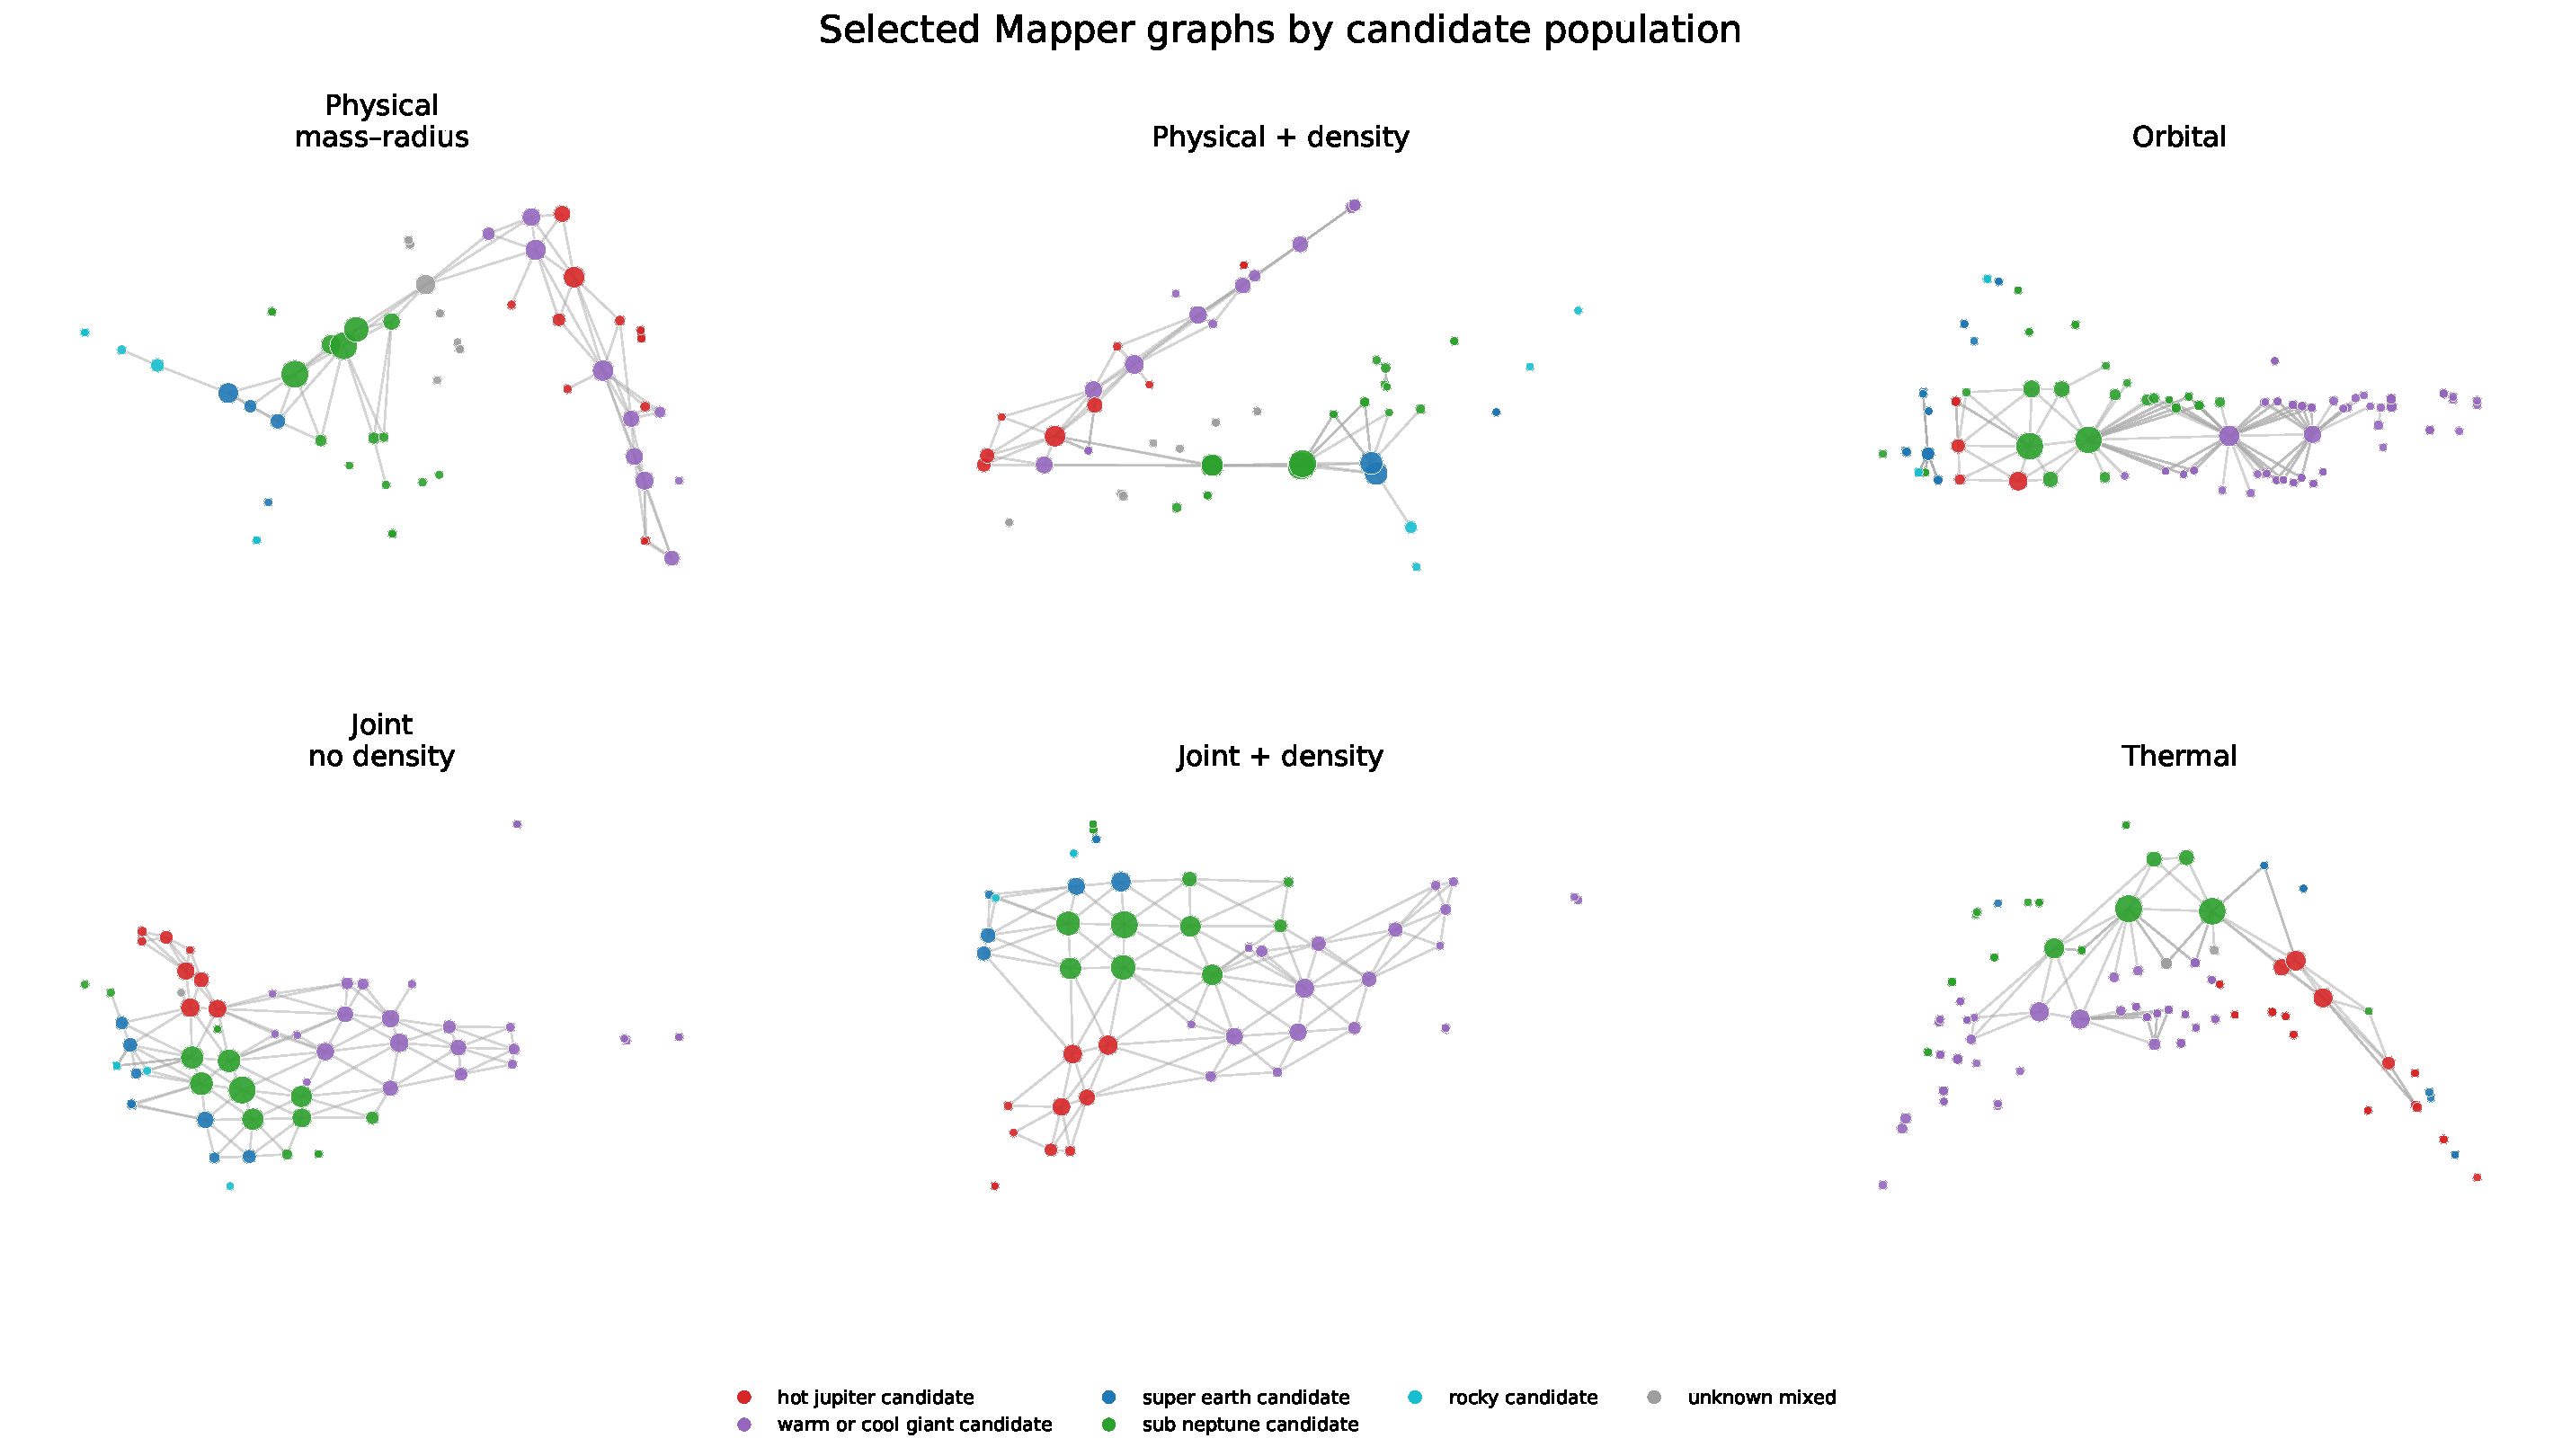
\includegraphics[width=0.92\linewidth]{figures/astro_main_graphs_by_candidate_population.pdf}
\caption{Grafos principales coloreados por población física heurística. La visualización permite evaluar si las regiones de Mapper están dominadas por poblaciones candidatas o si la señal física aparece mezclada dentro de los grafos. La presencia de grandes regiones dominadas por una misma etiqueta debe interpretarse como coherencia heurística local, no como una clase planetaria definitiva.}
\label{fig:main_graphs_by_population}
\end{figure}

\begin{figure}[H]
\centering
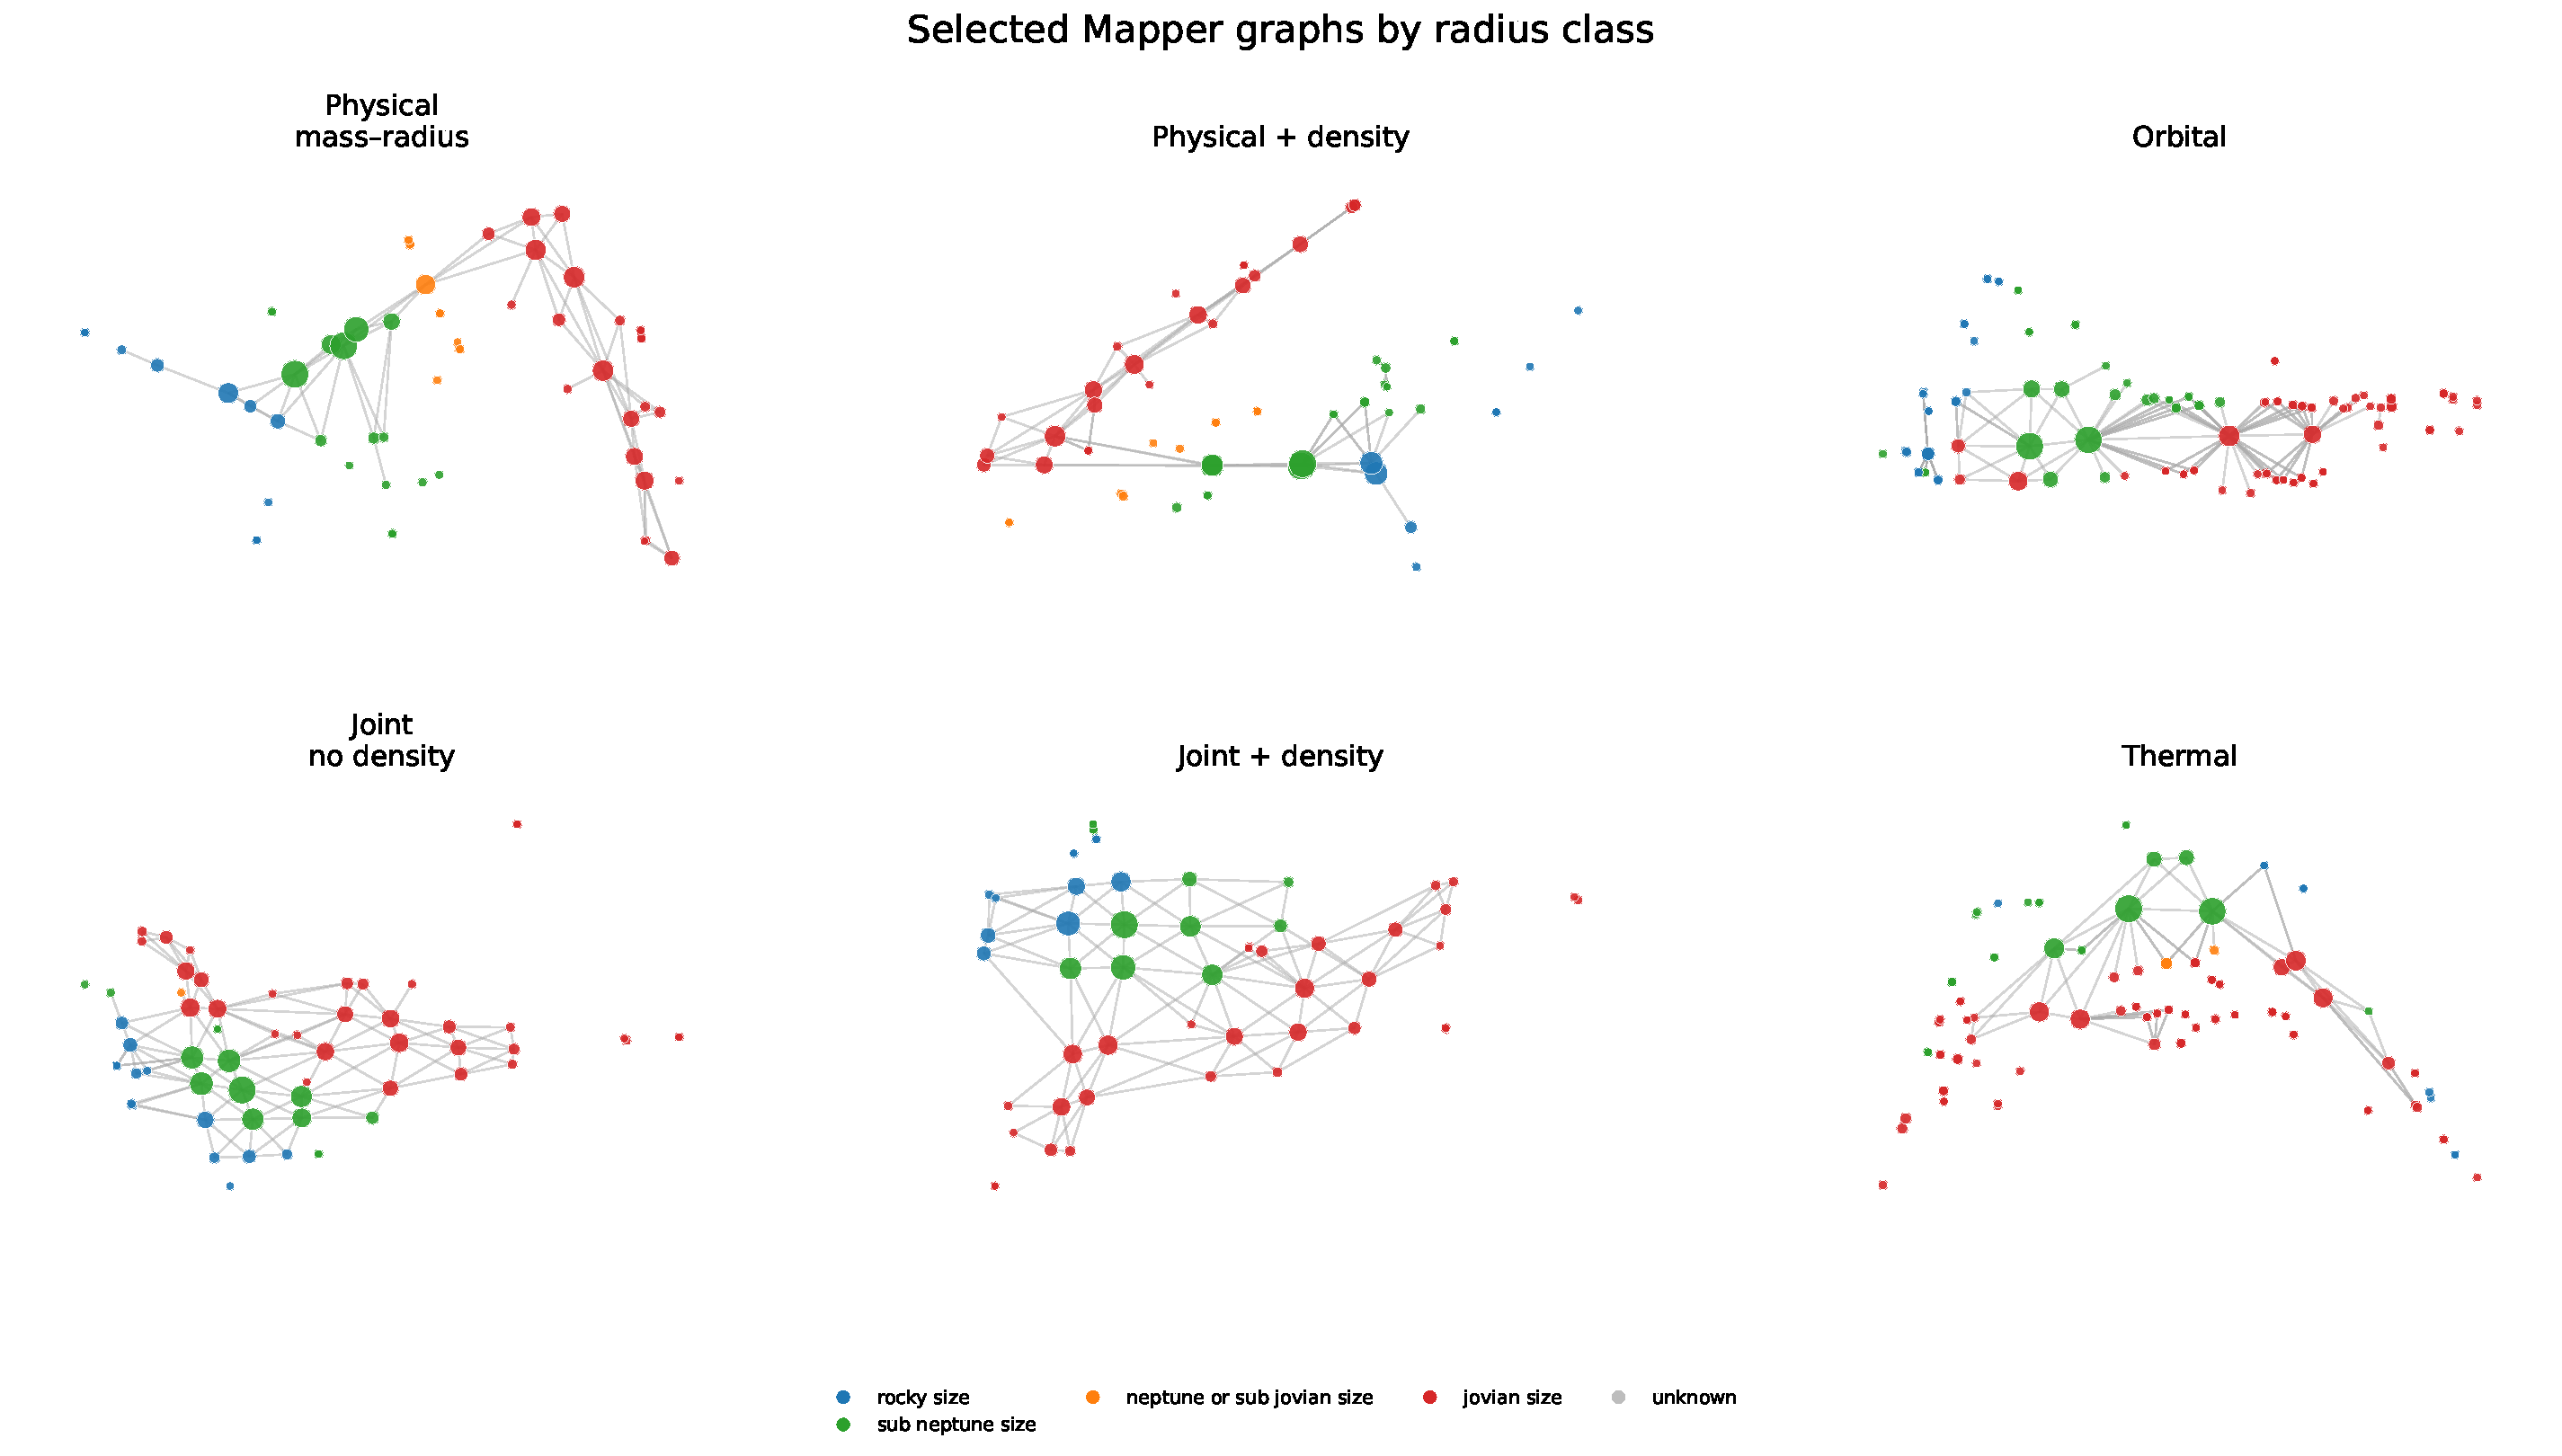
\includegraphics[width=0.92\linewidth]{figures/astro_main_graphs_by_radius_class.pdf}
\caption{Grafos principales coloreados por clase de radio dominante. Esta version separa visualmente regiones \texttt{rocky\_size}, \texttt{sub\_neptune\_size}, \texttt{neptune\_or\_sub\_jovian\_size} y \texttt{jovian\_size}, lo que permite revisar si la estructura local coincide con gradientes de tamano planetario.}
\label{fig:astro_main_graphs_by_radius_class}
\end{figure}

La Figura~\ref{fig:main_graphs_by_population} muestra que las etiquetas heurísticas pueden ayudar a ubicar regiones físicamente plausibles, pero también evidencia una limitación importante: en varios grafos la señal visual aparece concentrada en regiones grandes y no necesariamente separada en múltiples poblaciones limpias. Esto refuerza la idea de que la interpretación debe hacerse por región y no solo por inspección global del grafo. Una población heurística dominante puede indicar coherencia física local, pero todavía debe cruzarse con imputación y sesgo observacional.

Además de las clases por radio, los nodos físicos resumen valores medios y medianos de \texttt{pl\_rade}, \texttt{pl\_bmasse} y \texttt{pl\_dens}. Esto permite leer gradientes de tamaño, masa y densidad entre regiones del grafo. La densidad, sin embargo, requiere una interpretación particular. Aunque \texttt{pl\_dens} es físicamente útil para distinguir planetas compactos de planetas de baja densidad, muchos de sus valores fueron derivados a partir de masa y radio. Por ello, cuando se usa junto con \texttt{pl\_rade} y \texttt{pl\_bmasse}, no debe tratarse como evidencia completamente independiente.

\begin{figure}[H]
\centering
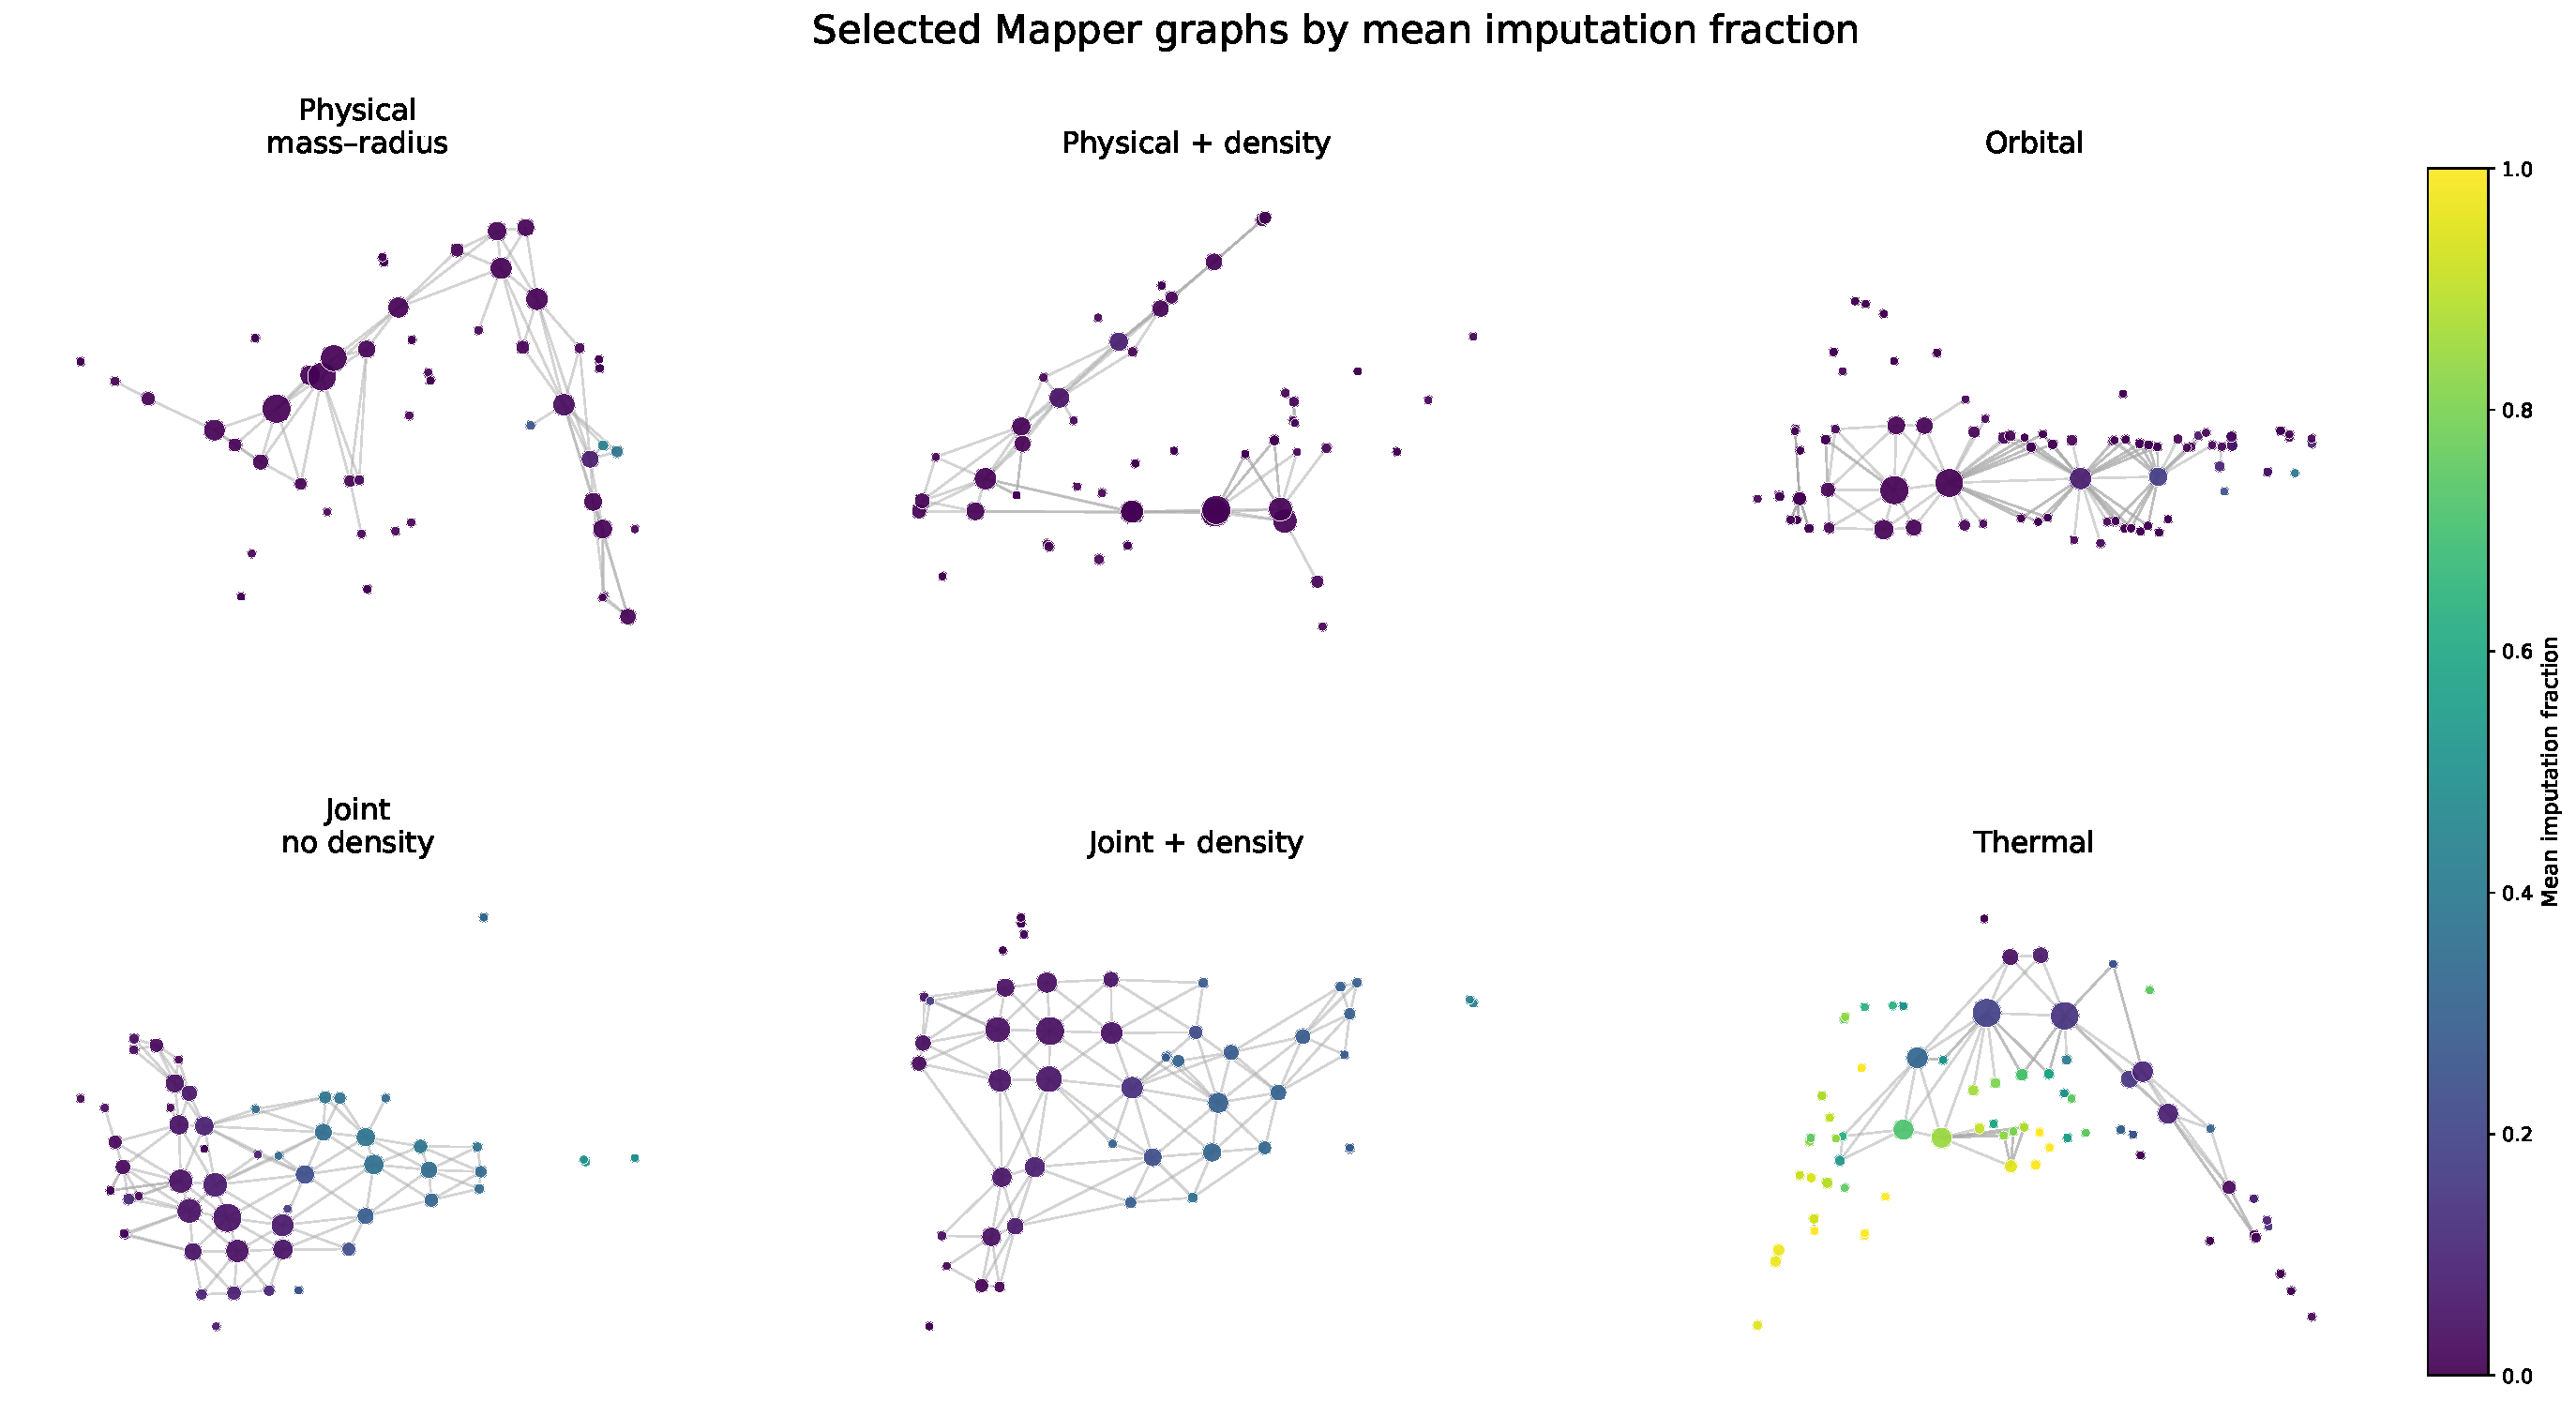
\includegraphics[width=0.92\linewidth]{figures/astro_main_graphs_by_imputation_fraction.pdf}
\caption{Grafos principales coloreados por fracción de imputación o trazabilidad de origen de datos. Esta visualización permite distinguir regiones sostenidas principalmente por datos observados de regiones con mayor dependencia de valores imputados o derivados. En particular, ayuda a interpretar con cautela los espacios que incorporan variables térmicas o densidad derivada.}
\label{fig:main_graphs_by_imputation}
\end{figure}

La Figura~\ref{fig:main_graphs_by_imputation} muestra por qué la interpretación astrofísica no puede separarse de la trazabilidad de datos. Una región puede parecer estructurada, pero si su color indica alta imputación o alta proporción de valores derivados, la evidencia que sostiene esa región es más débil. Esta observación es especialmente relevante para el espacio térmico y para los grafos que incorporan \texttt{pl\_dens}. En esos casos, la estructura observada puede ser útil como señal exploratoria, pero no debe elevarse directamente a conclusión física fuerte.

Los resultados medidos sugieren que la densidad actúa más como una variable de regularización que como una fuente nueva de ramificación topológica. Al comparar el espacio físico mínimo con el espacio físico con densidad, \(\beta_1\) baja de 54 en \texttt{phys\_min} a 52 en \texttt{phys\_density}. De manera similar, en el espacio conjunto \(\beta_1\) baja de 81 en \texttt{joint\_no\_density} a 77 en \texttt{joint}. Esta disminución indica que agregar \texttt{pl\_dens} compacta u ordena parte del espacio, en lugar de crear más ciclos o ramas. Por esta razón, los grafos con densidad se leen como controles metodológicos y no como evidencia independiente de una estructura física adicional.

La estructura orbital es el resultado más importante del análisis. El grafo \texttt{orbital\_pca2\_cubes10\_overlap0p35} tiene 124 nodos, 196 aristas, \(\beta_1=96\) e imputación media nodal de 0.011. Esta combinación lo vuelve el candidato más fuerte para inspección científica: muestra una topología rica y, al mismo tiempo, depende poco de valores imputados. Como este grafo usa \texttt{pl\_orbper} y \texttt{pl\_orbsmax}, su estructura es compatible con una organización del catálogo según escala orbital, es decir, por periodo y distancia media a la estrella.

Dentro de la lectura orbital, las etiquetas como \texttt{short\_period}, \texttt{intermediate\_period} y \texttt{long\_period} permiten distinguir regiones asociadas con distintos regímenes orbitales. Las regiones de periodo corto son físicamente interpretables porque corresponden a planetas cercanos a su estrella, pero también deben leerse con cuidado: los métodos de tránsito tienden a detectar con mayor facilidad planetas de periodos cortos. Por eso, una región dominada por planetas de periodo corto puede reflejar tanto una propiedad orbital real como un sesgo de observación.

También aparecen regiones compatibles con órbitas más amplias, incluyendo etiquetas como \texttt{long\_period} o poblaciones candidatas como \texttt{long\_period\_giant\_candidate}. Estas regiones son científicamente interesantes porque pueden señalar arquitecturas orbitales distintas, pero su composición también puede estar asociada con métodos específicos de detección, como imagen directa, microlente o velocidad radial. En consecuencia, la interpretación orbital debe mantenerse como una lectura mixta: el grafo muestra estructura, pero esa estructura puede combinar arquitectura orbital y selección observacional.

El espacio térmico presenta un caso distinto. El grafo \texttt{thermal\_pca2\_cubes10\_overlap0p35} tiene \(\beta_1=67\), lo que indica una estructura no trivial. Sin embargo, su imputación media nodal es 0.588 y la fracción de nodos con alta imputación es 0.719. Esto debilita significativamente su interpretación física. El espacio térmico puede sugerir gradientes energéticos relacionados con \texttt{pl\_insol} y \texttt{pl\_eqt}, pero no debe usarse como evidencia física fuerte sin una auditoría adicional de imputación. En este reporte, el grafo térmico funciona principalmente como caso de cautela metodológica: una estructura puede ser visualmente rica y, aun así, estar sostenida por datos completados estadísticamente.

Los espacios conjuntos permiten observar cómo se combinan propiedades físicas, orbitales y térmicas. En particular, \texttt{joint\_no\_density\_pca2\_cubes10\_overlap0p35} combina radio, masa, periodo, semieje mayor, insolación y temperatura de equilibrio. Este grafo tiene \(\beta_1=81\) e imputación media de 0.176. La complejidad del espacio conjunto sugiere que algunas regiones pueden alinear propiedades físicas y orbitales, pero la presencia de variables térmicas aumenta el riesgo por imputación. Por tanto, estas regiones se leen como candidatas mixtas: pueden ser astrofísicamente interesantes, pero requieren más cautela que el grafo orbital.

La síntesis final de regiones refuerza esta lectura cautelosa. La evidencia astrofísica más útil aparece cuando una región combina baja imputación, coherencia física u orbital y baja concentración observacional. Bajo estos criterios, los resultados finales identifican 10 nodos etiquetados como \texttt{physical}. Esto indica que existen regiones con evidencia relativamente limpia de interpretación física, pero son pocas en comparación con el total de regiones estructuradas. En contraste, muchas regiones quedan clasificadas como \texttt{mixed}: 240 nodos y 36 componentes. Esto significa que presentan algún patrón físico u orbital, pero también una señal observacional relevante.

Este resultado es importante porque cambia la lectura del proyecto. Si se observara únicamente la complejidad de los grafos, podría parecer tentador hablar de familias planetarias o de clases emergentes. Sin embargo, el predominio de regiones \texttt{mixed} muestra que la estructura observada no es puramente astrofísica ni puramente observacional. En muchos casos, Mapper detecta regiones donde la señal física u orbital está mezclada con método de descubrimiento, imputación, derivaciones físicas o sensibilidad metodológica.

Por esta razón, las regiones físicamente interpretables deben leerse como candidatas para inspección posterior. Una región con alta pureza de clase física, baja imputación y baja concentración por \texttt{discoverymethod} puede considerarse una candidata fuerte. En cambio, una región con coherencia física pero alta asociación con método de descubrimiento debe clasificarse como mixta. Esta clasificación no debilita el proyecto; al contrario, muestra por qué la auditoría era necesaria. Sin ella, una región estructurada podría haberse interpretado erróneamente como una familia física pura.

Una pregunta central de esta sección es si las regiones observadas pueden interpretarse como clases planetarias reales. La respuesta metodológica es no. Las regiones Mapper deben leerse como candidatos interpretativos, no como clases definitivas. Un nodo puede estar dominado por planetas pequeños, por gigantes o por un régimen orbital particular, pero su significado depende de la imputación, de la composición observacional y de la sensibilidad del lente. Esta cautela es especialmente importante porque la auditoría de sesgo observacional mostró asociación con \texttt{discoverymethod}. En el grafo orbital, por ejemplo, la pureza ponderada observada por método fue 0.842, el NMI observado fue 0.254 y el valor empírico de la prueba por permutación fue \(p=0.001\). Por ello, no se puede descartar que parte de la estructura orbital refleje sesgo de descubrimiento.

La dependencia de imputación también varía fuertemente entre espacios. El patrón orbital es menos dependiente de imputación que el térmico: la imputación media nodal del grafo orbital es 0.011, mientras que la del grafo térmico es 0.588. El espacio físico mínimo también tiene baja imputación, con 0.017, mientras que el espacio conjunto sin densidad tiene una imputación moderada de 0.176. Estas diferencias justifican que el grafo orbital y el físico mínimo se consideren más confiables que el térmico para interpretación inicial.

Finalmente, existen artefactos para tres lentes: \texttt{pca2}, \texttt{domain} y \texttt{density}. Sin embargo, la interpretación activa del reporte se basa en \texttt{pca2}. Las otras lentes funcionan como sensibilidad metodológica, no como confirmación definitiva. Además, como los artefactos reconciliados no constituyen una grilla completa de \texttt{n\_cubes} y \texttt{overlap}, la persistencia de patrones entre lentes debe leerse con cuidado. Hay evidencia para comparar lentes bajo una cubierta fija, pero no suficiente para afirmar robustez completa frente a todos los hiperparámetros de Mapper.

\subsection*{Visualizaciones astrofisicas complementarias}

Las siguientes figuras usan el mismo estilo de renderizado limpio que la sintesis final, pero colorean los grafos por etiquetas interpretativas astrofisicas. Estas visualizaciones no definen clases finales; sirven para ubicar regiones candidatas y compararlas con la auditoria de imputacion y sesgo observacional.

\begin{figure}[H]
\centering
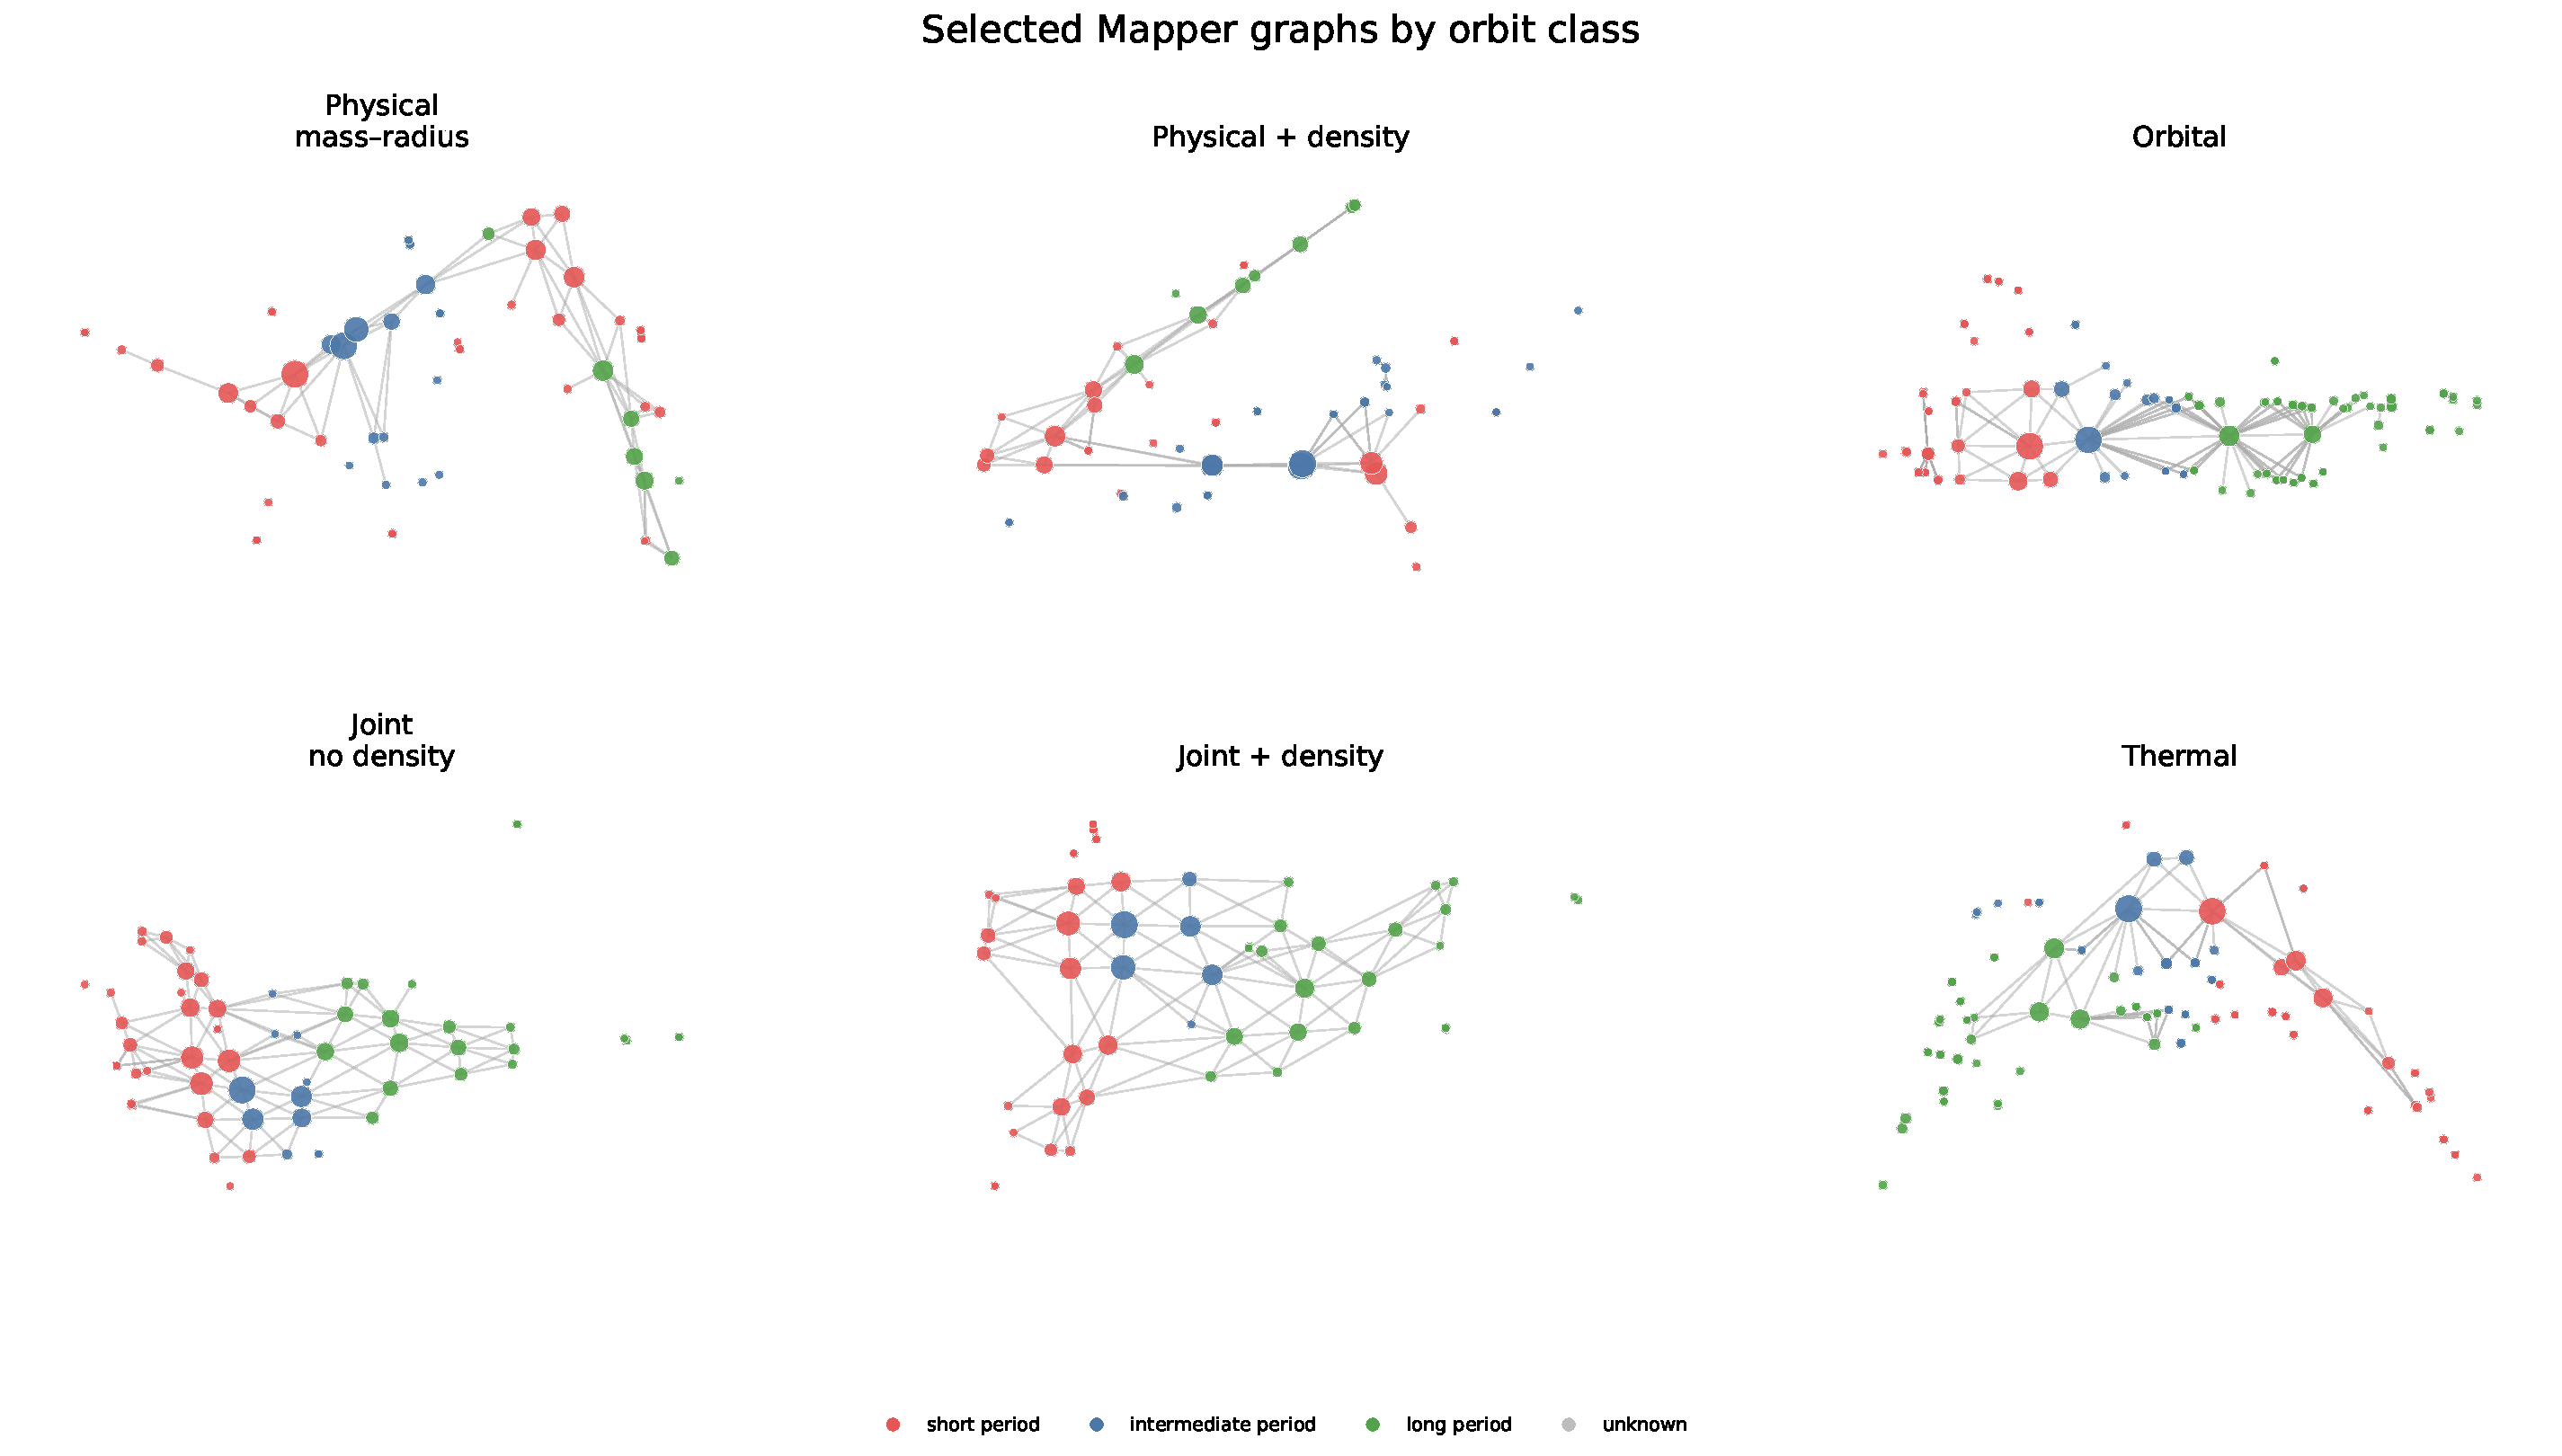
\includegraphics[width=0.92\linewidth]{figures/astro_main_graphs_by_orbit_class.pdf}
\caption{Grafos principales coloreados por clase orbital dominante. La figura permite comparar regiones de periodo corto, intermedio y largo en los espacios seleccionados.}
\label{fig:astro_main_graphs_by_orbit_class}
\end{figure}

\begin{figure}[H]
\centering
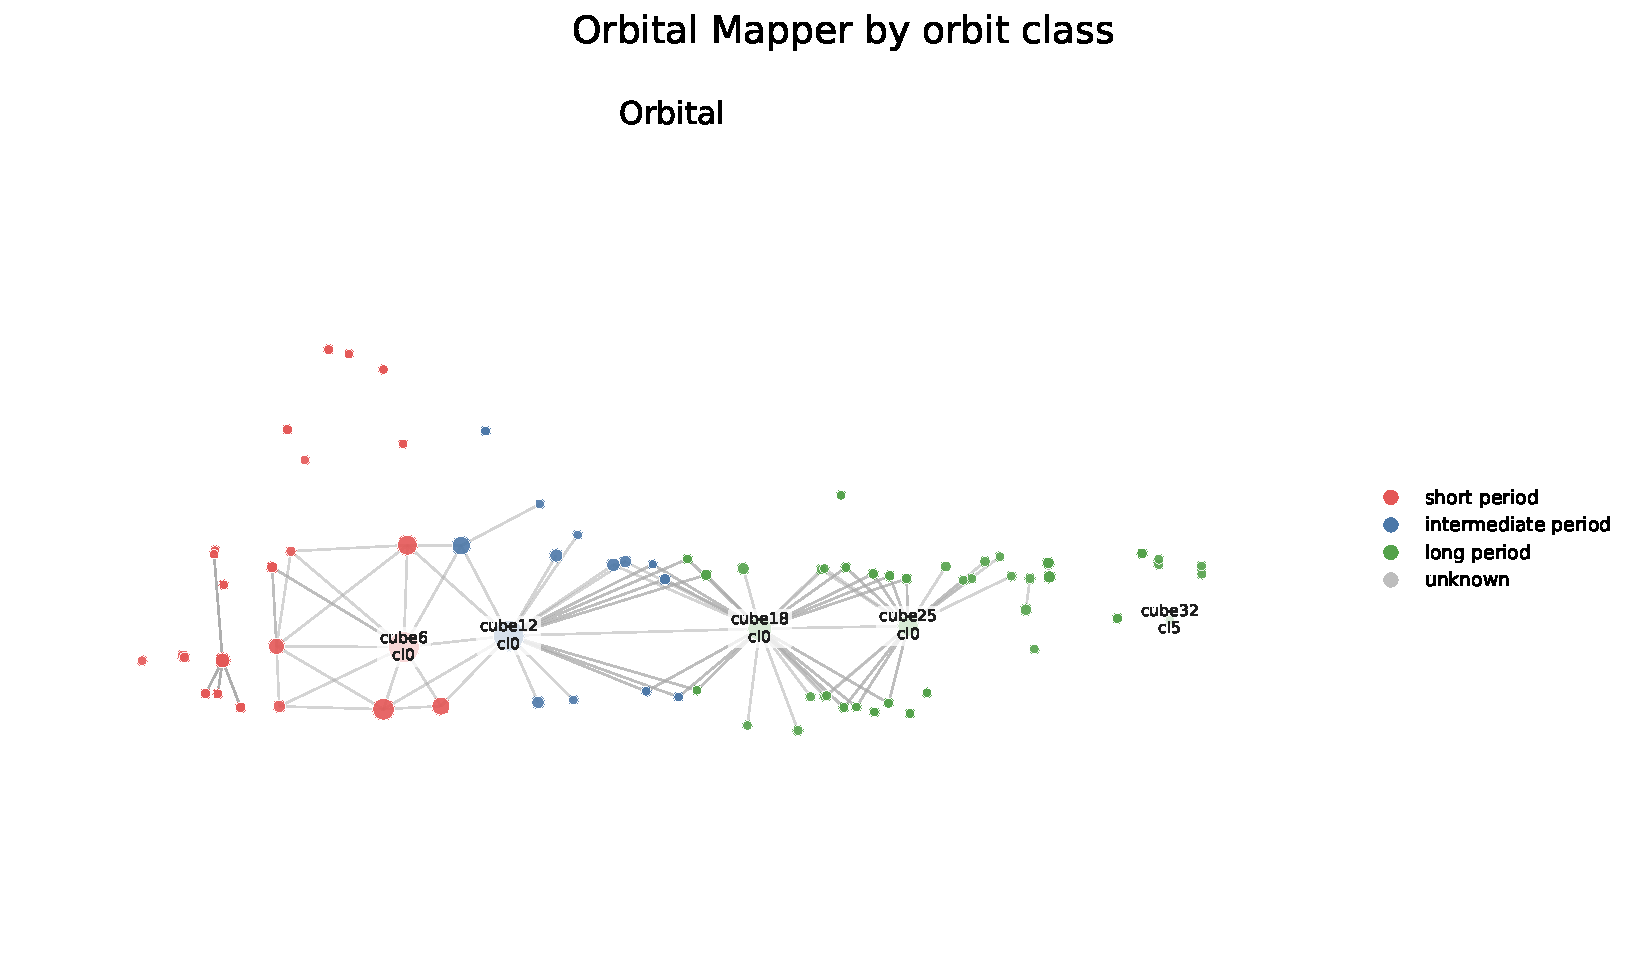
\includegraphics[width=0.78\linewidth]{figures/astro_orbital_graph_by_orbit_class.pdf}
\caption{Grafo orbital coloreado por clase orbital dominante. La figura muestra la transicion visual entre regiones de periodo corto, intermedio y largo.}
\label{fig:astro_orbital_graph_by_orbit_class}
\end{figure}

\begin{figure}[H]
\centering
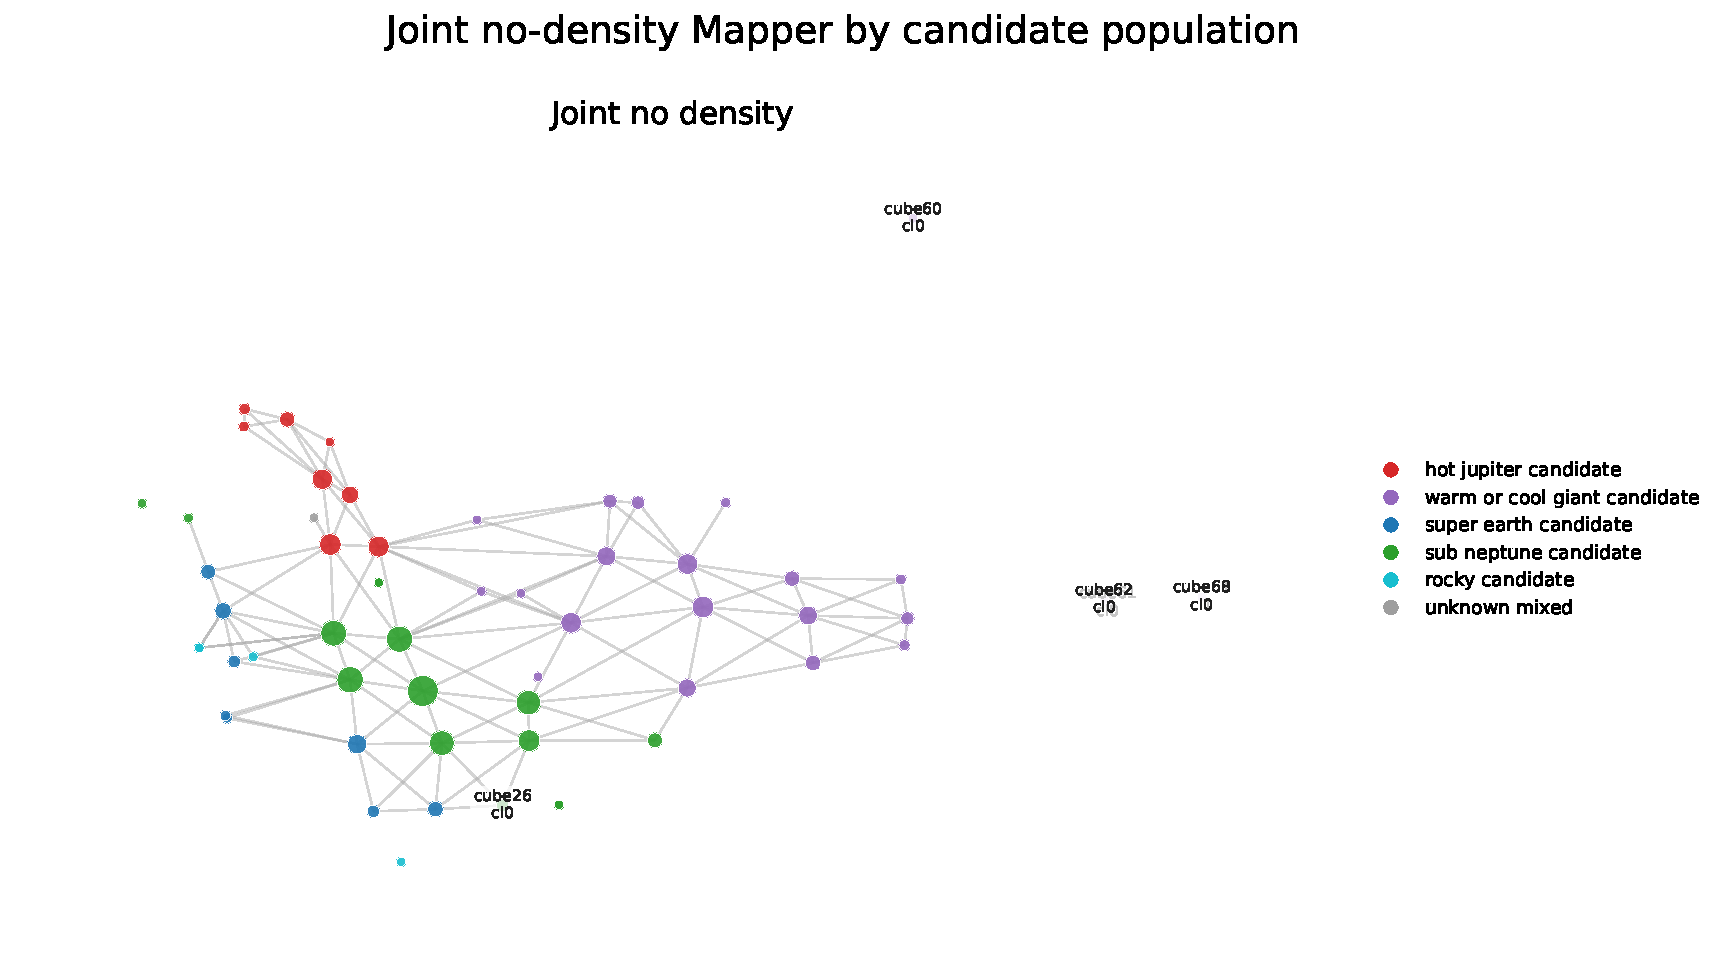
\includegraphics[width=0.78\linewidth]{figures/astro_joint_no_density_graph_by_candidate_population.pdf}
\caption{Grafo conjunto sin densidad coloreado por poblacion candidata. Esta vista ayuda a revisar donde se alinean radio, masa, orbita y variables termicas sin introducir la densidad derivada como coordenada adicional.}
\label{fig:astro_joint_no_density_graph_by_candidate_population}
\end{figure}

\begin{figure}[H]
\centering
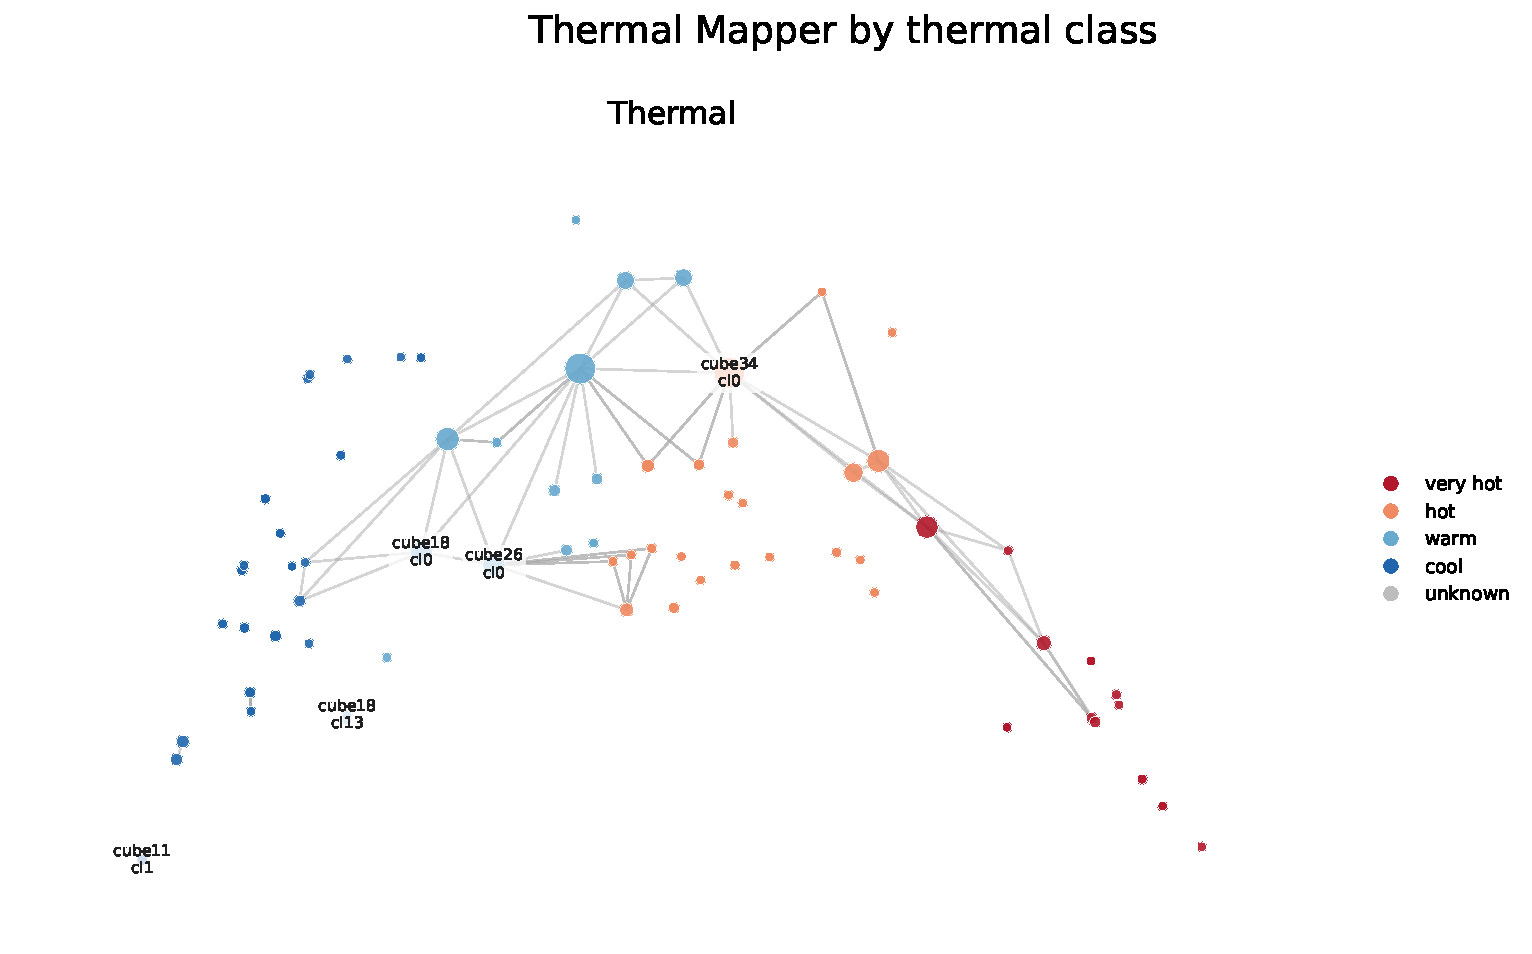
\includegraphics[width=0.78\linewidth]{figures/astro_thermal_graph_by_thermal_class.pdf}
\caption{Grafo termico coloreado por clase termica dominante. Aunque aparecen gradientes de temperatura, la alta imputacion del espacio termico obliga a leer esta estructura como evidencia cautelosa.}
\label{fig:astro_thermal_graph_by_thermal_class}
\end{figure}

\begin{table}[H]
\centering
\scriptsize
\caption{Comparacion de espacios de variables para los artefactos existentes.}
\label{tab:space_comparison}
\begin{adjustbox}{max width=\linewidth}
\begin{tabular}{llrrrr}
\toprule
feature\_space & lens & beta\_1 & n\_nodes & n\_edges & mean\_node\_imputation \\
\midrule
joint & density & 153 & 117 & 260 & 0.106 \\
joint\_no\_density & density & 134 & 109 & 233 & 0.142 \\
orb\_thermal & density & 138 & 121 & 246 & 0.255 \\
orbital & density & 144 & 178 & 297 & 0.030 \\
phys\_density & density & 52 & 78 & 109 & 0.002 \\
phys\_min & density & 75 & 97 & 152 & 0.010 \\
thermal & density & 171 & 205 & 338 & 0.472 \\
joint & domain & 59 & 64 & 116 & 0.121 \\
joint\_no\_density & domain & 0 & 9 & 0 & 0.212 \\
orb\_thermal & domain & 38 & 56 & 82 & 0.254 \\
orbital & domain & 42 & 77 & 94 & 0.034 \\
phys\_density & domain & 68 & 80 & 132 & 0.010 \\
phys\_min & domain & 64 & 76 & 125 & 0.010 \\
thermal & domain & 48 & 95 & 105 & 0.527 \\
joint & pca2 & 77 & 56 & 126 & 0.152 \\
joint\_no\_density & pca2 & 81 & 62 & 134 & 0.176 \\
orb\_thermal & pca2 & 54 & 58 & 100 & 0.347 \\
orbital & pca2 & 96 & 124 & 196 & 0.011 \\
phys\_density & pca2 & 52 & 67 & 102 & 0.002 \\
phys\_min & pca2 & 54 & 66 & 105 & 0.017 \\
thermal & pca2 & 67 & 121 & 150 & 0.588 \\
\bottomrule
\end{tabular}
\end{adjustbox}

\end{table}


En síntesis, la interpretación astrofísica más defendible es que los grafos Mapper revelan regiones candidatas, especialmente en el espacio orbital y en los espacios físicos de baja imputación. Algunas regiones son compatibles con clases por radio, gradientes masa-radio o regímenes orbitales. Sin embargo, esas regiones no son clases finales. Su interpretación debe cruzarse con tres auditorías: imputación, sesgo observacional y sensibilidad metodológica. Bajo esta lectura, el resultado principal no es una nueva taxonomía de exoplanetas, sino un conjunto de regiones candidatas que pueden clasificarse como físicas, observacionales, mixtas o débiles.

\section{Auditoria de sesgo observacional}
La auditoría de sesgo observacional se incorporó porque los exoplanetas no se descubren de manera uniforme. Cada método de detección favorece regiones distintas del espacio planetario. Por ejemplo, el método de tránsito detecta con mayor facilidad planetas de periodo corto, cercanos a su estrella, grandes y alineados con nuestra línea de visión. La velocidad radial favorece planetas masivos o de periodo moderado alrededor de estrellas donde la señal gravitacional sea medible. La imagen directa favorece planetas gigantes, jóvenes, calientes, luminosos y separados de su estrella. Por esta razón, una región Mapper puede aparecer no solamente porque los planetas sean físicamente parecidos, sino porque fueron detectados mediante un mismo procedimiento observacional.

En este reporte, las variables \texttt{discoverymethod}, \texttt{disc\_year} y \texttt{disc\_facility} se usan como metadata externa para auditar sesgo observacional. No son variables de entrada de Mapper. Esta decisión es metodológicamente importante: \texttt{discoverymethod} no describe qué es físicamente el planeta, sino cómo fue encontrado. Si se usara como coordenada del Mapper, podría contaminar la geometría del grafo y agrupar planetas por historia observacional en lugar de por propiedades físicas, orbitales o térmicas.

La pregunta de esta auditoría es entonces:

\begin{quote}
¿Las regiones del grafo Mapper están alineadas con propiedades físicas u orbitales, o están enriquecidas por el proceso de descubrimiento?
\end{quote}

Para responderla, se calculó la composición de cada nodo por método de descubrimiento. Para un nodo \(v\) con conjunto de miembros \(S_v\), la distribución por método se define como:

\[
p_v(m)=\frac{|\{i\in S_v : d_i=m\}|}{|S_v|},
\]

donde \(d_i\) es el método de descubrimiento del planeta \(i\), y \(m\) recorre los métodos observados en el catálogo. A partir de esta distribución se calculó la pureza por método:

\[
P_v = \max_m p_v(m),
\]

que mide la fracción del método dominante dentro del nodo. Si \(P_v=1\), todos los planetas del nodo fueron descubiertos por el mismo método. Si \(P_v\) es menor, el nodo mezcla varios métodos.

También se calculó la entropía por método:

\[
H_v=-\sum_m p_v(m)\log p_v(m).
\]

La entropía mide qué tan mezclados están los métodos de descubrimiento dentro del nodo. Una entropía baja indica dominancia de un método; una entropía alta indica una composición más diversa. Por lo tanto, un nodo con pureza alta y entropía baja es observacionalmente más sospechoso que un nodo con mezcla de métodos.

Además de pureza y entropía, se evaluó la divergencia entre la composición local del nodo y la composición global del catálogo. Esta comparación es necesaria porque algunos métodos, como tránsito, pueden ser frecuentes en el catálogo completo. Un nodo con muchos planetas de tránsito no es necesariamente sorprendente si el catálogo global ya está dominado por tránsito. En cambio, un nodo cuya composición por método se aleja fuertemente de la distribución global muestra enriquecimiento local por método de descubrimiento.

Las variables \texttt{disc\_year} y \texttt{disc\_facility} añaden una capa temporal e instrumental a la auditoría. \texttt{disc\_year} permite detectar si una región está concentrada en una época de descubrimiento, mientras que \texttt{disc\_facility} permite identificar regiones dominadas por una misión, telescopio o instalación específica. Si un nodo está dominado simultáneamente por un método, una facilidad y una ventana temporal estrecha, la evidencia de sesgo observacional se vuelve más fuerte.

Una región se considera observacionalmente sospechosa cuando presenta una o varias de las siguientes señales:

\begin{itemize}
    \item alta pureza por \texttt{discoverymethod};
    \item baja entropía por método;
    \item alta divergencia respecto a la distribución global del catálogo;
    \item dominancia de una sola \texttt{disc\_facility};
    \item concentración en una ventana estrecha de \texttt{disc\_year};
    \item enriquecimiento significativo en la prueba de permutación.
\end{itemize}

Es importante subrayar que esta asociación no prueba causalidad. Un nodo dominado por \texttt{Transit}, \texttt{Radial Velocity} o \texttt{Imaging} no demuestra por sí mismo que el método haya causado la estructura. Sin embargo, sí indica que la región debe interpretarse con cautela, porque puede estar mezclando señal astrofísica con selección observacional.

\subsection*{Nodos enriquecidos por método de descubrimiento}

La auditoría identificó nodos con enriquecimiento fuerte por \texttt{discoverymethod}. Los casos más extremos aparecen en los grafos conjuntos y están dominados por \texttt{Imaging}. Por ejemplo, varios nodos en \texttt{joint\_pca2} y \texttt{joint\_no\_density\_pca2} presentan fracción dominante igual a 1.000, valores \(Z\) muy altos y \(p=0.001\). Estos nodos son especialmente sospechosos porque \texttt{Imaging} no observa uniformemente toda la población planetaria: tiende a favorecer planetas gigantes, jóvenes, luminosos y separados de su estrella.

\begin{table}[H]
\centering
\scriptsize
\caption{Nodos con mayor enriquecimiento por metodo de descubrimiento.}
\label{tab:top_enriched_nodes}
\begin{adjustbox}{max width=\linewidth}
\begin{tabular}{lllrrrr}
\toprule
config\_id & node\_id & dominant\_discoverymethod & observed\_dominant\_method\_fraction & enrichment\_z & empirical\_p\_value & n\_members \\
\midrule
joint\_pca2\_cubes10\_overlap0p35 & cube61\_cluster0 & Imaging & 1.000 & 46.721 & 0.001 & 8 \\
joint\_no\_density\_pca2\_cubes10\_overlap0p35 & cube61\_cluster0 & Imaging & 1.000 & 46.556 & 0.001 & 10 \\
joint\_pca2\_cubes10\_overlap0p35 & cube62\_cluster0 & Imaging & 1.000 & 39.721 & 0.001 & 5 \\
joint\_pca2\_cubes10\_overlap0p35 & cube47\_cluster0 & Imaging & 1.000 & 39.001 & 0.001 & 7 \\
joint\_pca2\_cubes10\_overlap0p35 & cube54\_cluster0 & Imaging & 1.000 & 39.001 & 0.001 & 7 \\
joint\_pca2\_cubes10\_overlap0p35 & cube48\_cluster1 & Imaging & 1.000 & 34.440 & 0.001 & 6 \\
joint\_pca2\_cubes10\_overlap0p35 & cube55\_cluster0 & Imaging & 1.000 & 34.440 & 0.001 & 6 \\
orbital\_pca2\_cubes10\_overlap0p35 & cube6\_cluster0 & Transit & 0.928 & 32.343 & 0.001 & 3316 \\
joint\_no\_density\_pca2\_cubes10\_overlap0p35 & cube61\_cluster1 & Imaging & 1.000 & 29.951 & 0.001 & 4 \\
joint\_no\_density\_pca2\_cubes10\_overlap0p35 & cube62\_cluster0 & Imaging & 1.000 & 29.951 & 0.001 & 4 \\
joint\_no\_density\_pca2\_cubes10\_overlap0p35 & cube68\_cluster0 & Imaging & 1.000 & 29.951 & 0.001 & 4 \\
thermal\_pca2\_cubes10\_overlap0p35 & cube26\_cluster0 & Radial Velocity & 0.586 & 29.905 & 0.001 & 720 \\
joint\_no\_density\_pca2\_cubes10\_overlap0p35 & cube50\_cluster0 & Imaging & 1.000 & 29.623 & 0.001 & 5 \\
joint\_no\_density\_pca2\_cubes10\_overlap0p35 & cube51\_cluster0 & Imaging & 1.000 & 29.623 & 0.001 & 5 \\
joint\_no\_density\_pca2\_cubes10\_overlap0p35 & cube59\_cluster0 & Imaging & 1.000 & 29.623 & 0.001 & 5 \\
\bottomrule
\end{tabular}
\end{adjustbox}
\vspace{0.4em}\begin{minipage}{0.96\linewidth}\footnotesize Se muestran 15 de 496 filas; el CSV fuente contiene la tabla completa.\end{minipage}
\end{table}


La Tabla anterior debe leerse como una lista de regiones donde la topología local se alinea fuertemente con el método de descubrimiento. En particular, los nodos dominados por \texttt{Imaging} en los espacios conjuntos no deben interpretarse directamente como una población física limpia. Pueden ser científicamente interesantes, porque corresponden a planetas con propiedades extremas o poco comunes, pero su composición está fuertemente condicionada por el método que permitió detectarlos.

En el grafo orbital también aparecen nodos relevantes. Algunos nodos están dominados por \texttt{Transit}, como \texttt{cube6\_cluster0}, con fracción dominante de 0.928, y \texttt{cube12\_cluster0}, con fracción dominante de 0.877. Estos nodos son importantes porque el grafo orbital usa \texttt{pl\_orbper} y \texttt{pl\_orbsmax}; justamente las variables orbitales pueden estar muy ligadas al sesgo de tránsito, que favorece planetas cercanos y de periodo corto. Por lo tanto, una región orbital dominada por \texttt{Transit} puede reflejar una combinación de arquitectura orbital real y sesgo de detección.

También aparecen casos orbitales dominados por \texttt{Radial Velocity}, como \texttt{cube25\_cluster0}, con fracción dominante de 0.605, y nodos pequeños con presencia de \texttt{Imaging}, como \texttt{cube32\_cluster5}. Estos ejemplos no tienen la misma lectura que los nodos grandes dominados por tránsito: su tamaño, imputación y composición deben revisarse antes de asignarles una interpretación fuerte. En particular, los nodos pequeños pueden mostrar pureza alta simplemente por bajo número de miembros, por lo que deben leerse como señales de auditoría y no como evidencia concluyente.

\subsection*{Componentes enriquecidos}

La auditoría también se realizó a nivel de componentes conectadas. Esta escala es útil porque un componente puede reunir varios nodos relacionados y mostrar si una porción completa del grafo está dominada por un método de descubrimiento. Los componentes más sospechosos son aquellos pequeños o medianos dominados completamente por un solo método.

\begin{table}[H]
\centering
\scriptsize
\caption{Componentes con mayor concentracion observacional.}
\label{tab:component_discovery_bias}
\begin{adjustbox}{max width=\linewidth}
\begin{tabular}{lrrlrrlr}
\toprule
config\_id & component\_id & n\_members & dominant\_discoverymethod & dominant\_discoverymethod\_fraction & discoverymethod\_entropy & dominant\_disc\_facility & disc\_year\_median \\
\midrule
joint\_no\_density\_pca2\_cubes10\_overlap0p35 & 6 & 5 & Imaging & 1.000 & -0.000 & European Space Agency (ESA) Gaia Satellite & 2019.000 \\
joint\_no\_density\_pca2\_cubes10\_overlap0p35 & 7 & 10 & Imaging & 1.000 & -0.000 & W. M. Keck Observatory & 2018.000 \\
joint\_no\_density\_pca2\_cubes10\_overlap0p35 & 8 & 4 & Imaging & 1.000 & -0.000 & Paranal Observatory & 2016.500 \\
joint\_pca2\_cubes10\_overlap0p35 & 5 & 7 & Imaging & 1.000 & -0.000 & European Space Agency (ESA) Gaia Satellite & 2019.000 \\
joint\_pca2\_cubes10\_overlap0p35 & 6 & 8 & Imaging & 1.000 & -0.000 & Paranal Observatory & 2018.000 \\
thermal\_pca2\_cubes10\_overlap0p35 & 12 & 5 & Imaging & 0.600 & 1.371 & Multiple Observatories & 2023.000 \\
orbital\_pca2\_cubes10\_overlap0p35 & 18 & 4 & Microlensing & 0.500 & 1.500 & KMTNet & 2020.500 \\
thermal\_pca2\_cubes10\_overlap0p35 & 13 & 4 & Radial Velocity & 0.750 & 0.811 & European Space Agency (ESA) Gaia Satellite & 2015.000 \\
orbital\_pca2\_cubes10\_overlap0p35 & 23 & 4 & Imaging & 0.500 & 1.500 & Hubble Space Telescope & 2014.500 \\
thermal\_pca2\_cubes10\_overlap0p35 & 6 & 8 & Radial Velocity & 0.875 & 0.544 & La Silla Observatory & 2014.000 \\
thermal\_pca2\_cubes10\_overlap0p35 & 15 & 6 & Microlensing & 0.667 & 0.918 & KMTNet & 2023.000 \\
orbital\_pca2\_cubes10\_overlap0p35 & 13 & 5 & Radial Velocity & 0.800 & 0.722 & Multiple Observatories & 2014.000 \\
thermal\_pca2\_cubes10\_overlap0p35 & 3 & 10 & Radial Velocity & 0.900 & 0.469 & Multiple Observatories & 2010.000 \\
orbital\_pca2\_cubes10\_overlap0p35 & 12 & 5 & Radial Velocity & 1.000 & -0.000 & La Silla Observatory & 2011.000 \\
orbital\_pca2\_cubes10\_overlap0p35 & 14 & 4 & Radial Velocity & 1.000 & -0.000 & W. M. Keck Observatory & 2017.000 \\
\bottomrule
\end{tabular}
\end{adjustbox}
\vspace{0.4em}\begin{minipage}{0.96\linewidth}\footnotesize Se muestran 15 de 110 filas; el CSV fuente contiene la tabla completa.\end{minipage}
\end{table}


En los resultados, varios componentes de \texttt{joint\_no\_density\_pca2} y \texttt{joint\_pca2} aparecen completamente dominados por \texttt{Imaging}. Algunos de ellos tienen además imputación moderada o alta, por ejemplo componentes con imputación de 0.333, 0.500, 0.286 o 0.429. Esta combinación es importante: cuando una región está dominada por un método de descubrimiento y además depende de imputación, su interpretación física se debilita. En esos casos, la región debe clasificarse con mayor probabilidad como observacional o mixta.

En el grafo orbital también pueden existir componentes dominados por \texttt{Transit} o \texttt{Radial Velocity}. Sin embargo, varios de esos componentes son pequeños, por lo que funcionan mejor como alertas de auditoría que como conclusiones fuertes. Esta diferencia muestra por qué la auditoría debe combinar varias métricas: pureza, entropía, divergencia, tamaño del nodo o componente, imputación y contexto astrofísico.

\subsection*{Lectura metodológica de la auditoría}

La conclusión principal de esta auditoría es que varias regiones Mapper están significativamente enriquecidas por método de descubrimiento. Esto no invalida los grafos, pero sí cambia su interpretación. Una estructura topológica puede ser informativa y, al mismo tiempo, estar parcialmente asociada con la manera en que los planetas fueron detectados.

En particular, las regiones conjuntas dominadas por \texttt{Imaging} y las regiones orbitales dominadas por \texttt{Transit} deben interpretarse como evidencia mixta: potencialmente astrofísica, pero también observacionalmente sesgada. Esta lectura es más fuerte que simplemente aceptar o rechazar el grafo. Permite separar regiones con señal física más limpia de regiones donde la topología observada puede estar influida por el catálogo.

Por lo tanto, la auditoría de sesgo observacional funciona como un filtro de interpretación. Una región con coherencia física, baja imputación y baja concentración por método puede considerarse una candidata más robusta. Una región con coherencia física pero alta dominancia por \texttt{discoverymethod} debe leerse como mixta. Una región dominada por método, facilidad o época, y además con alta imputación, debe leerse como observacional o débil.

Esta etapa es central para el objetivo del proyecto: no basta con encontrar estructura en Mapper; hay que evaluar si esa estructura se sostiene como señal astrofísica o si refleja el proceso de observación. Bajo esta lectura, el reporte no propone una taxonomía final de exoplanetas, sino una clasificación crítica de regiones candidatas según la evidencia que las sostiene.
\section{Prueba nula por permutacion de discoverymethod}
La auditoría por \texttt{discoverymethod} identifica nodos y componentes dominados por ciertos métodos de descubrimiento. Sin embargo, esa observación por sí sola no basta: si un método es muy frecuente en el catálogo global, algunos nodos podrían parecer dominados por ese método simplemente por azar. Por esta razón, se implementó una prueba nula por permutación.

La hipótesis nula de esta prueba es que las etiquetas \texttt{discoverymethod} no están asociadas de forma especial con la estructura Mapper. En otras palabras, si los métodos de descubrimiento se repartieran aleatoriamente entre los mismos planetas, los nodos no deberían mostrar una concentración por método mayor que la esperada bajo azar.

La prueba mantiene fija toda la estructura de Mapper: la topología del grafo, los nodos, las aristas y la membresía de planetas en cada nodo. El Mapper no se vuelve a correr. Lo único que se permuta son las etiquetas \texttt{discoverymethod} entre planetas. Esto permite construir escenarios nulos donde los mismos nodos existen, con los mismos planetas y la misma distribución global de métodos, pero sin asociación específica entre método de descubrimiento y posición topológica.

Esta decisión es importante. Si se permutaran las variables físicas u orbitales, cambiaría la geometría del problema y se estaría evaluando otra cosa. Aquí la pregunta es más precisa: dado el grafo Mapper observado, ¿la concentración de métodos de descubrimiento dentro de sus nodos es mayor que la esperada por azar?

Para cada nodo \(v\), se compara la pureza observada por método con la distribución nula obtenida por permutación. El estadístico reportado es:

\[
Z_v =
\frac{
P_v^{obs}-\mathbb{E}[P_v^{null}]
}{
\operatorname{sd}(P_v^{null})+\epsilon
}.
\]

Aquí \(P_v^{obs}\) es la pureza observada del nodo, \(\mathbb{E}[P_v^{null}]\) es la pureza promedio esperada bajo permutaciones, \(\operatorname{sd}(P_v^{null})\) es su desviación estándar y \(\epsilon\) es un término pequeño para evitar división entre cero. Un valor \(Z_v\) alto indica que la concentración observada por método es mucho mayor que la esperada bajo la hipótesis nula.

Además de los enriquecimientos por nodo, se calcularon estadísticos globales por grafo. Los principales fueron: la pureza media ponderada por tamaño de nodo, la entropía media ponderada y la información mutua normalizada, o NMI, entre una asignación dura de planeta a nodo y \texttt{discoverymethod}.

NMI se interpreta aquí como una medida de cuánta información comparte la posición de un planeta en el grafo con su método de descubrimiento. Si el NMI observado es alto en comparación con la distribución nula, entonces saber en qué nodo cae un planeta ayuda a predecir con qué método fue descubierto. Como Mapper permite que un planeta pertenezca a varios nodos, se construyó una asignación dura determinista: cada planeta se asignó al nodo más grande al que pertenece; en caso de empate, se usó el orden alfabético del identificador del nodo.

La auditoría final se realizó con 1000 permutaciones. Por lo tanto, valores empíricos como \(p=0.001\) indican evidencia fuerte de asociación bajo la resolución de esta prueba. Esta evidencia no prueba causalidad, pero sí muestra que la alineación entre topología y método de descubrimiento es demasiado fuerte para atribuirla fácilmente al azar.

\begin{table}[H]
\centering
\scriptsize
\caption{Prueba nula por permutacion de etiquetas discoverymethod.}
\label{tab:bias_permutation_null}
\begin{adjustbox}{max width=\linewidth}
\begin{tabular}{lrrrrrrrr}
\toprule
config\_id & observed\_weighted\_mean\_method\_purity & null\_mean\_purity & purity\_z & purity\_empirical\_p & observed\_nmi & null\_mean\_nmi & nmi\_z & nmi\_empirical\_p \\
\midrule
phys\_min\_pca2\_cubes10\_overlap0p35 & 0.765 & 0.730 & 12.961 & 0.001 & 0.136 & 0.009 & 131.786 & 0.001 \\
phys\_density\_pca2\_cubes10\_overlap0p35 & 0.783 & 0.731 & 21.768 & 0.001 & 0.150 & 0.009 & 136.246 & 0.001 \\
orbital\_pca2\_cubes10\_overlap0p35 & 0.842 & 0.773 & 26.630 & 0.001 & 0.254 & 0.009 & 209.663 & 0.001 \\
joint\_no\_density\_pca2\_cubes10\_overlap0p35 & 0.851 & 0.748 & 37.830 & 0.001 & 0.226 & 0.009 & 233.752 & 0.001 \\
joint\_pca2\_cubes10\_overlap0p35 & 0.848 & 0.746 & 38.754 & 0.001 & 0.221 & 0.009 & 232.721 & 0.001 \\
thermal\_pca2\_cubes10\_overlap0p35 & 0.813 & 0.756 & 20.860 & 0.001 & 0.207 & 0.012 & 147.018 & 0.001 \\
\bottomrule
\end{tabular}
\end{adjustbox}

\end{table}


La Tabla anterior resume los resultados globales de la prueba por permutación para los grafos seleccionados. El caso más importante para la interpretación del reporte es \texttt{orbital\_pca2\_cubes10\_overlap0p35}, porque este grafo fue identificado como el candidato estructural principal por su alta complejidad topológica y baja imputación.

Para el grafo orbital, la pureza media ponderada observada por método fue 0.842, mientras que la media nula de pureza fue 0.773. El valor \texttt{purity\_z} fue 26.630 y el valor empírico fue \(p=0.001\). Esto indica que los nodos del grafo orbital están más concentrados por método de descubrimiento de lo esperado bajo permutación aleatoria.

El resultado es todavía más claro en NMI. El NMI observado para el grafo orbital fue 0.254, mientras que el NMI nulo medio fue 0.009. El valor \texttt{nmi\_z} fue 209.663 y el valor empírico fue \(p=0.001\). En términos interpretativos, esto significa que la asignación de planetas a nodos en el grafo orbital contiene información significativa sobre \texttt{discoverymethod}. Es decir, la topología orbital no es independiente del proceso de descubrimiento.

Este resultado debe leerse con cuidado. No significa que el grafo orbital sea únicamente un artefacto observacional. El mismo grafo tiene \(\beta_1=96\), imputación media nodal de 0.011 y está construido con variables físicamente relevantes, \texttt{pl\_orbper} y \texttt{pl\_orbsmax}. Por lo tanto, sigue siendo el candidato más informativo para inspección científica. Sin embargo, la prueba de permutación muestra que su estructura no puede interpretarse como señal orbital pura.

La conclusión adecuada es mixta. El Mapper orbital revela una estructura rica y de baja imputación, compatible con organización por escala orbital, pero esa estructura también está fuertemente asociada con el método de descubrimiento. Esto es astrofísicamente razonable: los métodos de tránsito favorecen planetas cercanos y de periodo corto, mientras que otros métodos, como velocidad radial o imagen directa, favorecen distintas regiones del espacio orbital y físico. Por tanto, parte de la topología orbital puede reflejar arquitectura planetaria y parte puede reflejar selección observacional.

Esta prueba nula cumple una función central en el reporte. Sin ella, una región dominada por planetas orbitalmente parecidos podría interpretarse demasiado rápido como una población física. Con la permutación, en cambio, se puede distinguir entre regiones con señal más limpia y regiones donde la topología está significativamente alineada con \texttt{discoverymethod}. Por ello, los resultados de esta sección alimentan directamente la síntesis final de regiones: una región con coherencia física u orbital pero enriquecimiento significativo por método debe clasificarse como \texttt{mixed}, no como puramente física.

En resumen, la prueba por permutación muestra que la topología Mapper contiene asociación medible con el proceso de descubrimiento. Esta asociación no invalida el análisis, pero sí limita el tipo de conclusión que puede formularse. El resultado principal no es que Mapper descubra una topología orbital pura, sino que identifica una estructura exploratoria donde se mezclan señal orbital, sesgo observacional y decisiones de procesamiento. Esa es precisamente la razón por la que el reporte adopta una clasificación final de regiones físicas, observacionales, mixtas o débiles.





\section{Sintesis final de regiones}
La síntesis final clasifica las regiones Mapper según el tipo de evidencia que las sostiene. Esta clasificación no se aplica a planetas individuales ni busca construir una taxonomía final de exoplanetas. En cambio, clasifica nodos y componentes del grafo como regiones de evidencia: algunas tienen una interpretación física u orbital más limpia, otras están dominadas por variables observacionales, otras mezclan señal astrofísica y sesgo de descubrimiento, y otras no tienen suficiente soporte para ser interpretadas con confianza.

La pregunta central de esta sección es:

\begin{quote}
Después de construir Mapper, auditar imputación y auditar sesgo observacional, ¿qué tipo de regiones encontramos realmente?
\end{quote}

Para responderla, cada región se evaluó combinando cuatro fuentes de evidencia: coherencia física, orbital o térmica; enriquecimiento por \texttt{discoverymethod}; riesgo de imputación; y tamaño o confiabilidad de la región. Esta lectura permite evitar una interpretación demasiado directa de los grafos. Una región puede verse estructurada en Mapper, pero si está dominada por un método de descubrimiento, por una instalación específica o por valores altamente imputados, su interpretación astrofísica debe moderarse.

Las categorías finales son:

\begin{itemize}
    \item \texttt{physical}: regiones con coherencia física u orbital, baja imputación y baja evidencia de sesgo observacional.
    \item \texttt{observational}: regiones dominadas por método de descubrimiento, facilidad, época o enriquecimiento observacional significativo.
    \item \texttt{mixed}: regiones con alguna coherencia física u orbital, pero también con señal observacional relevante.
    \item \texttt{weak}: regiones con alta imputación, tamaño pequeño, evidencia conflictiva o soporte insuficiente para una interpretación fuerte.
\end{itemize}

Estas etiquetas no son clases planetarias. Son categorías de evidencia. Por ejemplo, una región \texttt{physical} no significa que se descubrió una nueva familia de planetas, sino que esa región tiene evidencia relativamente limpia para inspección astrofísica posterior. Del mismo modo, una región \texttt{mixed} no significa que no tenga señal física; significa que esa señal aparece entrelazada con sesgo observacional o incertidumbre metodológica.

\begin{table}[H]
\centering
\small
\begin{tabular}{lrrp{0.43\textwidth}}
\toprule
\textbf{Categoría} & \textbf{Nodos} & \textbf{Componentes} & \textbf{Lectura} \\
\midrule
\texttt{physical} & 10 & 0 & Regiones con evidencia física u orbital relativamente limpia. \\
\texttt{observational} & 1 & 4 & Regiones dominadas por señal observacional. \\
\texttt{mixed} & 240 & 36 & Regiones con señal física/orbital mezclada con sesgo observacional. \\
\texttt{weak} & 245 & 70 & Regiones con evidencia insuficiente, alta imputación o interpretación débil. \\
\bottomrule
\end{tabular}
\caption{Conteo final de regiones Mapper por tipo de evidencia.}
\label{tab:final_region_counts}
\end{table}

La Tabla~\ref{tab:final_region_counts} muestra que la mayor parte de la estructura no cae en una categoría puramente física. Solo 10 nodos fueron clasificados como \texttt{physical}, mientras que 240 nodos quedaron como \texttt{mixed} y 245 como \texttt{weak}. A nivel de componentes, predominan nuevamente las regiones \texttt{mixed} y \texttt{weak}. Esta distribución es uno de los resultados más importantes del proyecto: la topología observada no debe interpretarse como señal astrofísica limpia en bloque. Más bien, debe leerse como una mezcla de estructura física u orbital, sesgo observacional, imputación y sensibilidad metodológica.

\begin{figure}[H]
\centering
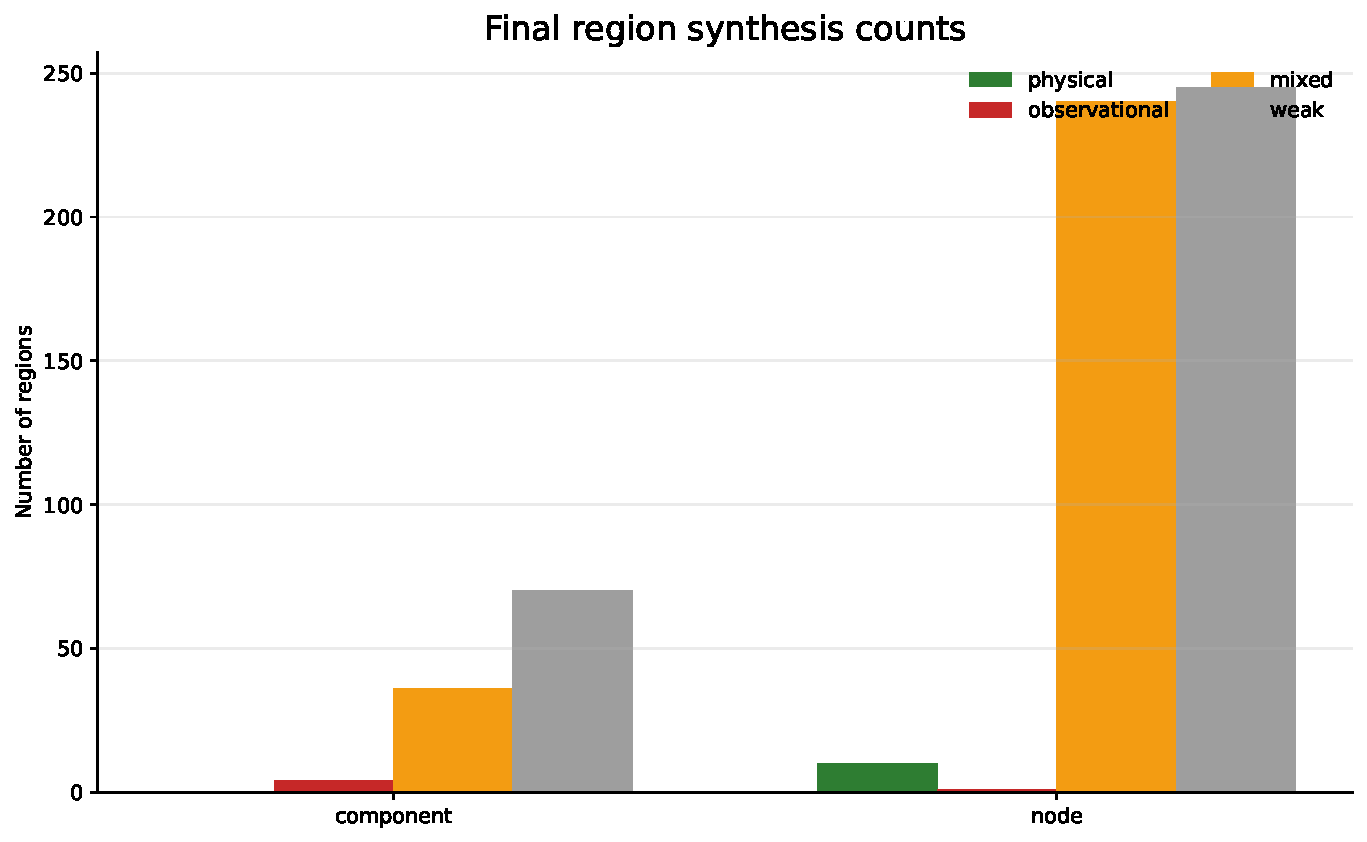
\includegraphics[width=0.78\linewidth]{figures/region_class_counts.pdf}
\caption{Conteos finales de regiones Mapper por categoría de evidencia. La figura resume la diferencia entre regiones \texttt{physical}, \texttt{observational}, \texttt{mixed} y \texttt{weak} a nivel de nodos y componentes.}
\label{fig:region_class_counts}
\end{figure}

La Figura~\ref{fig:region_class_counts} deja claro que el resultado dominante no es una colección de regiones físicas limpias, sino una abundancia de regiones mixtas y débiles. Esto no debilita el proyecto; al contrario, muestra que la auditoría era necesaria. Sin esta clasificación, sería fácil sobreinterpretar regiones estructuradas como familias planetarias, cuando en realidad muchas de ellas combinan señal física con sesgo de detección o incertidumbre de imputación.

\subsection*{Visualización de las regiones por tipo de evidencia}

La clasificación final también puede observarse directamente sobre los grafos seleccionados. La Figura~\ref{fig:main_graphs_by_evidence_class} muestra los seis grafos principales coloreados por categoría final de evidencia. Esta visualización permite comparar en una sola imagen qué tipo de regiones dominan en cada espacio de variables.

\begin{figure}[H]
\centering
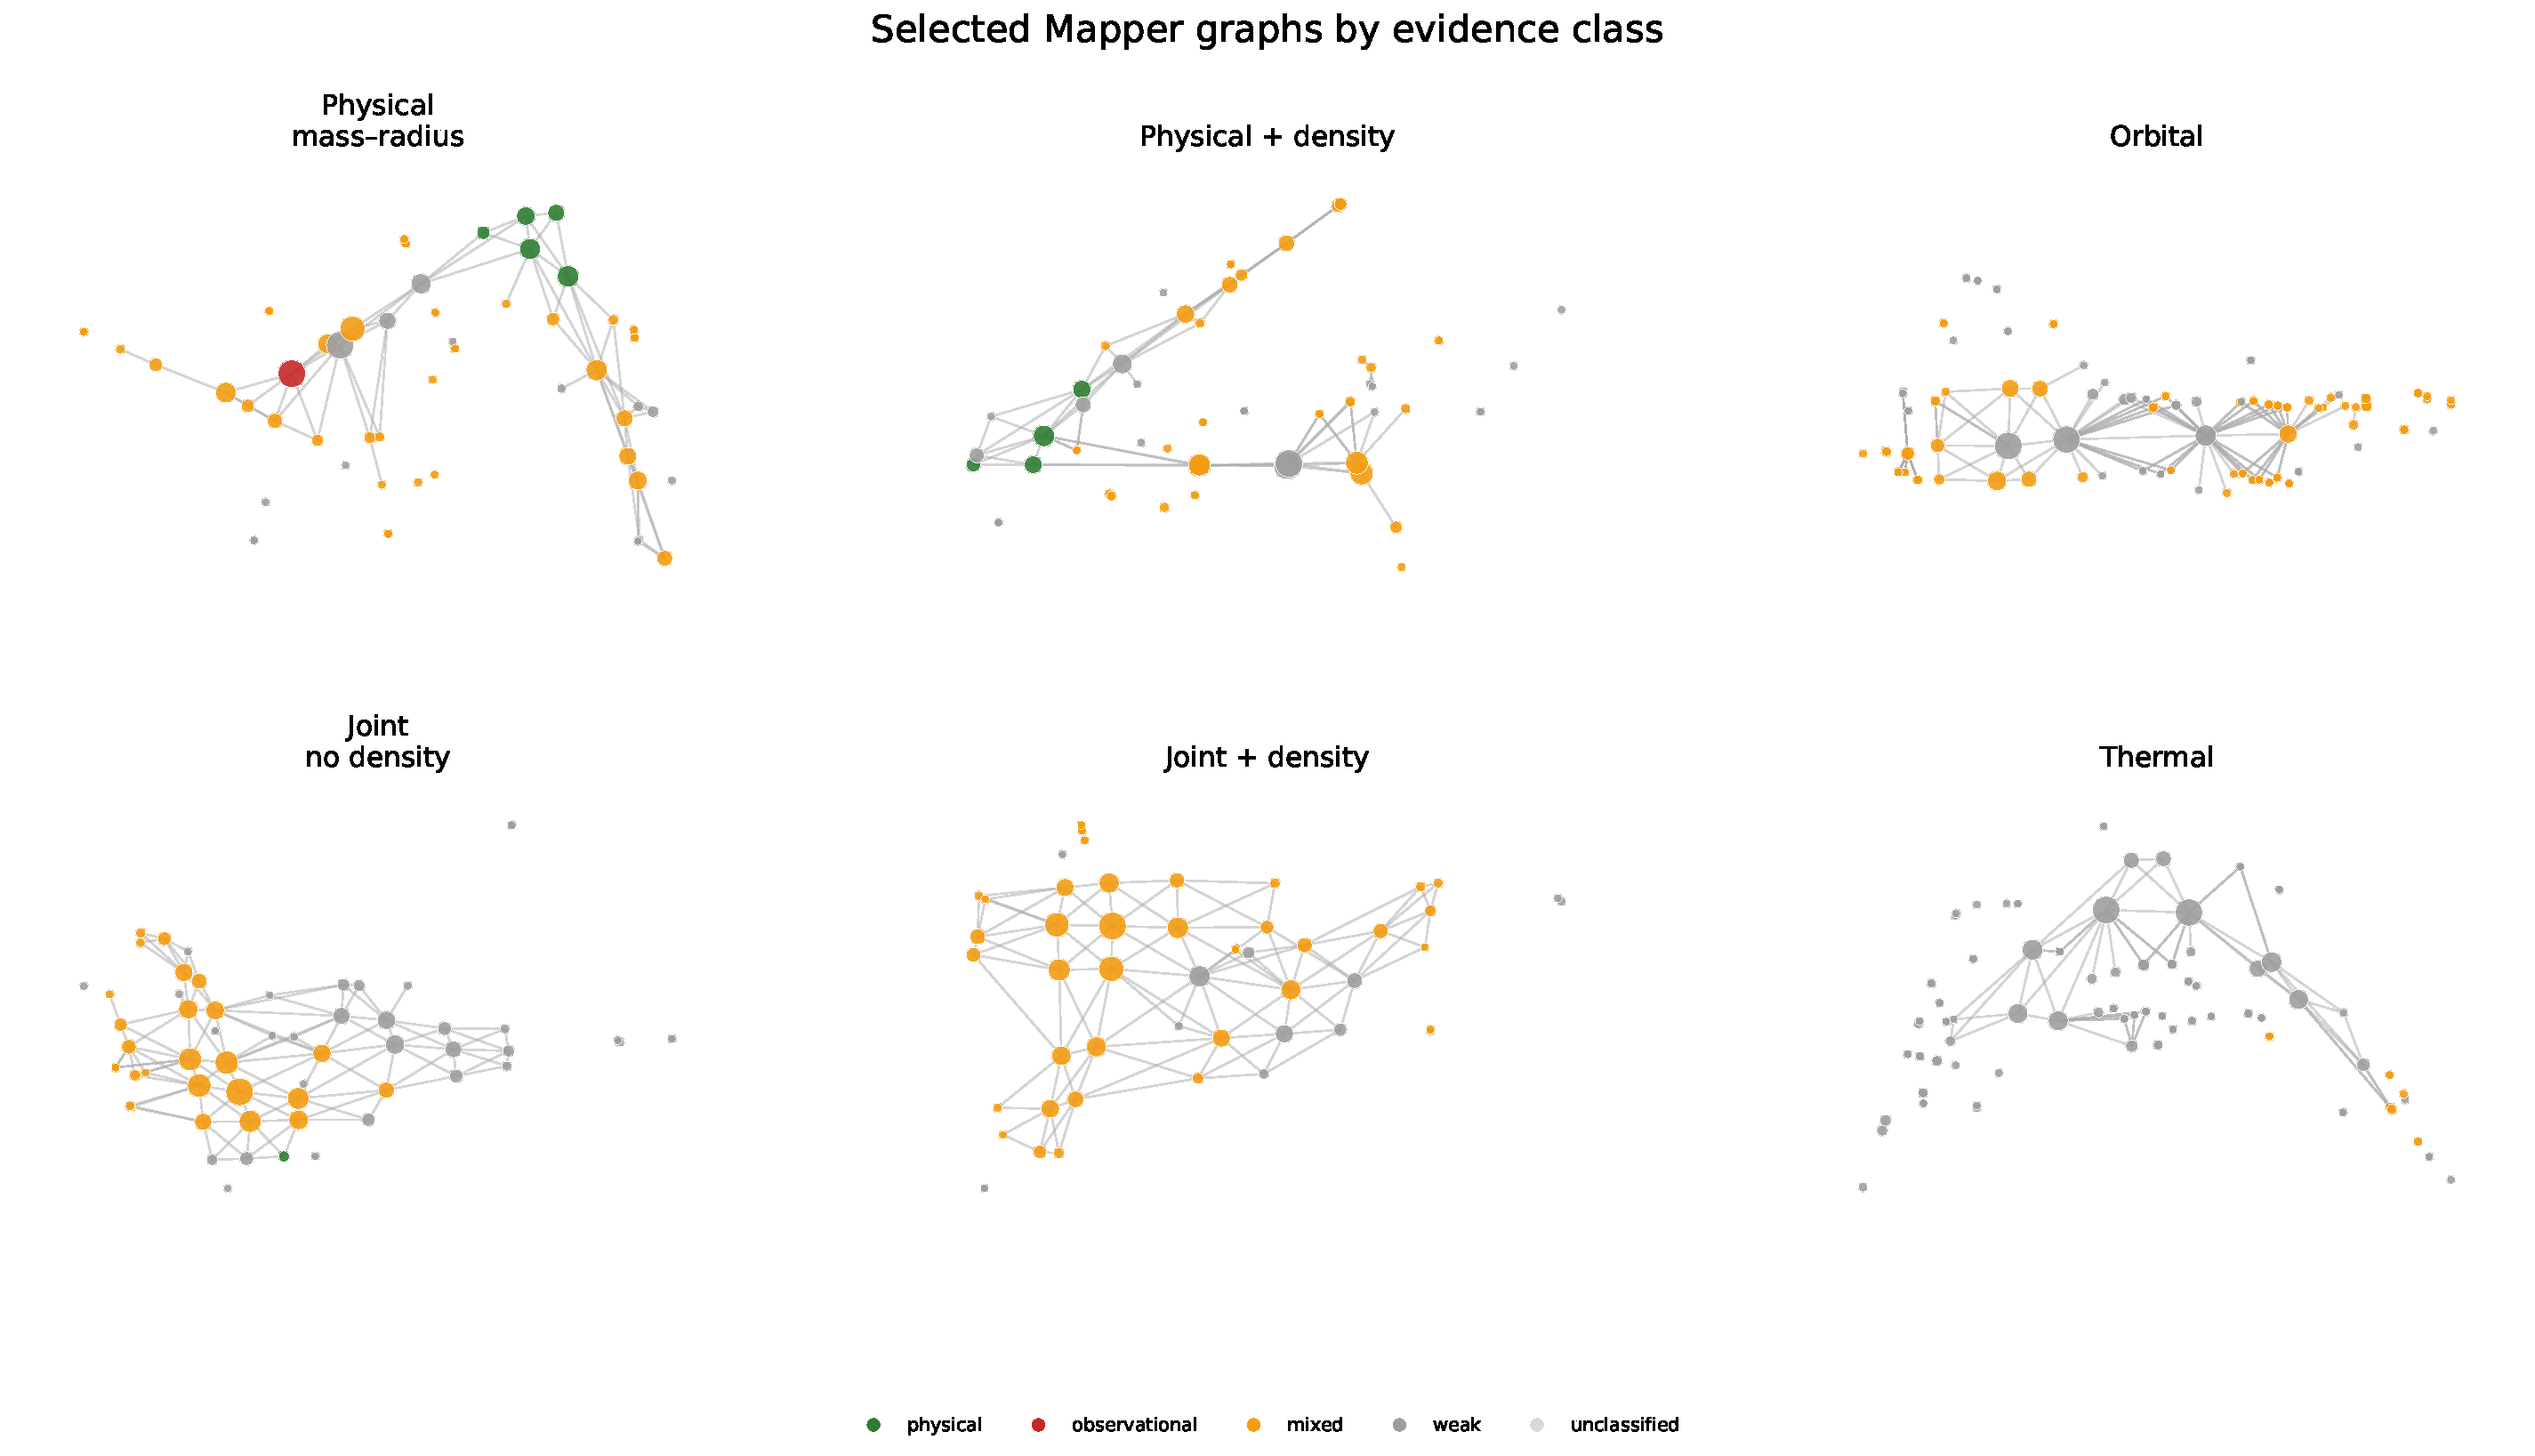
\includegraphics[width=0.95\linewidth]{figures/main_graphs_by_evidence_class.pdf}
\caption{Grafos Mapper seleccionados coloreados por categoría final de evidencia. Los colores distinguen regiones \texttt{physical}, \texttt{observational}, \texttt{mixed} y \texttt{weak}. La figura muestra que la estructura observada está dominada por regiones mixtas y débiles, mientras que las regiones físicas limpias son más escasas.}
\label{fig:main_graphs_by_evidence_class}
\end{figure}

La Figura~\ref{fig:main_graphs_by_evidence_class} es especialmente útil porque desplaza la lectura desde ``qué grafo se ve más complejo'' hacia ``qué tipo de evidencia sostiene cada región''. Un grafo puede tener muchos nodos y ciclos, pero si la mayoría de sus regiones son \texttt{mixed} o \texttt{weak}, la interpretación debe ser cautelosa. En cambio, las regiones \texttt{physical} son más valiosas como candidatas para inspección posterior porque combinan coherencia física u orbital con menor riesgo observacional y de imputación.

\subsection*{El caso del grafo orbital}

El grafo orbital sigue siendo el candidato principal del proyecto porque combina alta complejidad topológica con baja imputación. Tiene 124 nodos, 196 aristas, \(\beta_1=96\) e imputación media nodal de 0.011. Sin embargo, la síntesis final muestra que su interpretación no puede ser puramente astrofísica. La auditoría de \texttt{discoverymethod} mostró que su estructura tiene asociación significativa con el método de descubrimiento; por tanto, muchas regiones orbitales deben leerse como \texttt{mixed}.

\begin{figure}[H]
\centering
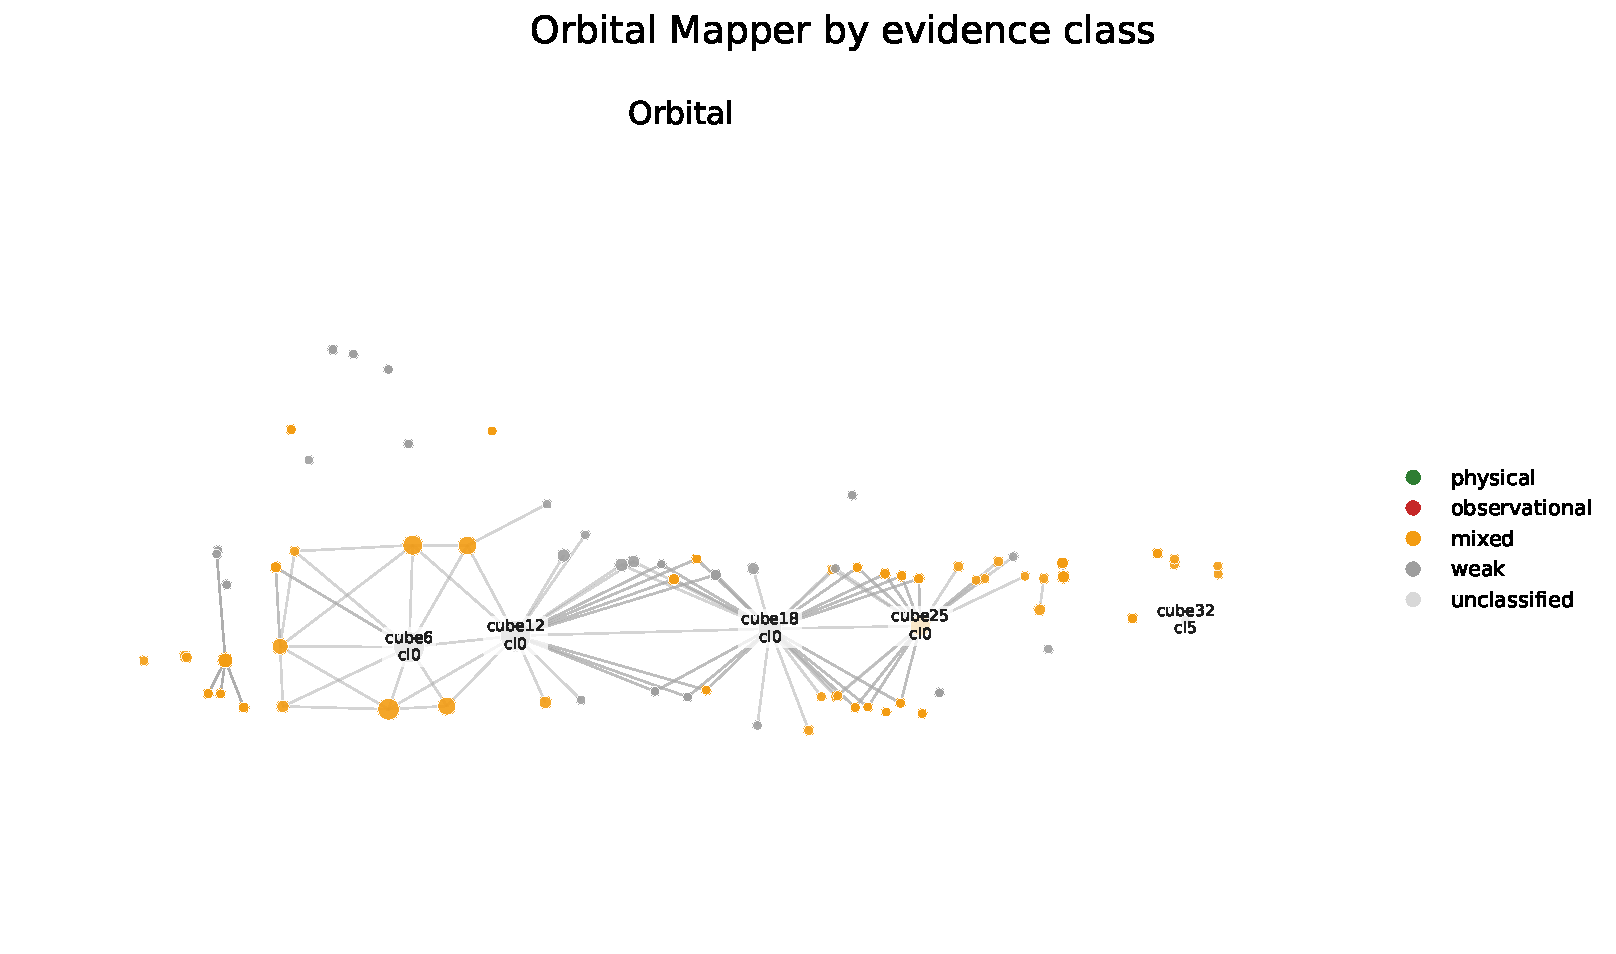
\includegraphics[width=0.78\linewidth]{figures/orbital_graph_evidence_class.pdf}
\caption{Grafo \texttt{orbital\_pca2\_cubes10\_overlap0p35} coloreado por categoría final de evidencia. Aunque el grafo orbital es el candidato más informativo por complejidad e imputación baja, muchas de sus regiones se interpretan como mixtas y no como señal orbital pura.}
\label{fig:orbital_graph_evidence_class}
\end{figure}

La Figura~\ref{fig:orbital_graph_evidence_class} muestra que el grafo orbital no debe resumirse simplemente como ``estructura física'' o ``sesgo''. Su valor está precisamente en la combinación: presenta estructura orbital informativa, pero esa estructura se intersecta con el proceso de descubrimiento. Esta lectura es consistente con el catálogo de exoplanetas: los planetas de periodo corto son más fáciles de detectar por tránsito, mientras que otros métodos favorecen regiones distintas del espacio físico y orbital.

Para distinguir mejor esa mezcla, se comparan dos visualizaciones adicionales del mismo grafo orbital: una por método de descubrimiento y otra por imputación.

\begin{figure}[H]
\centering
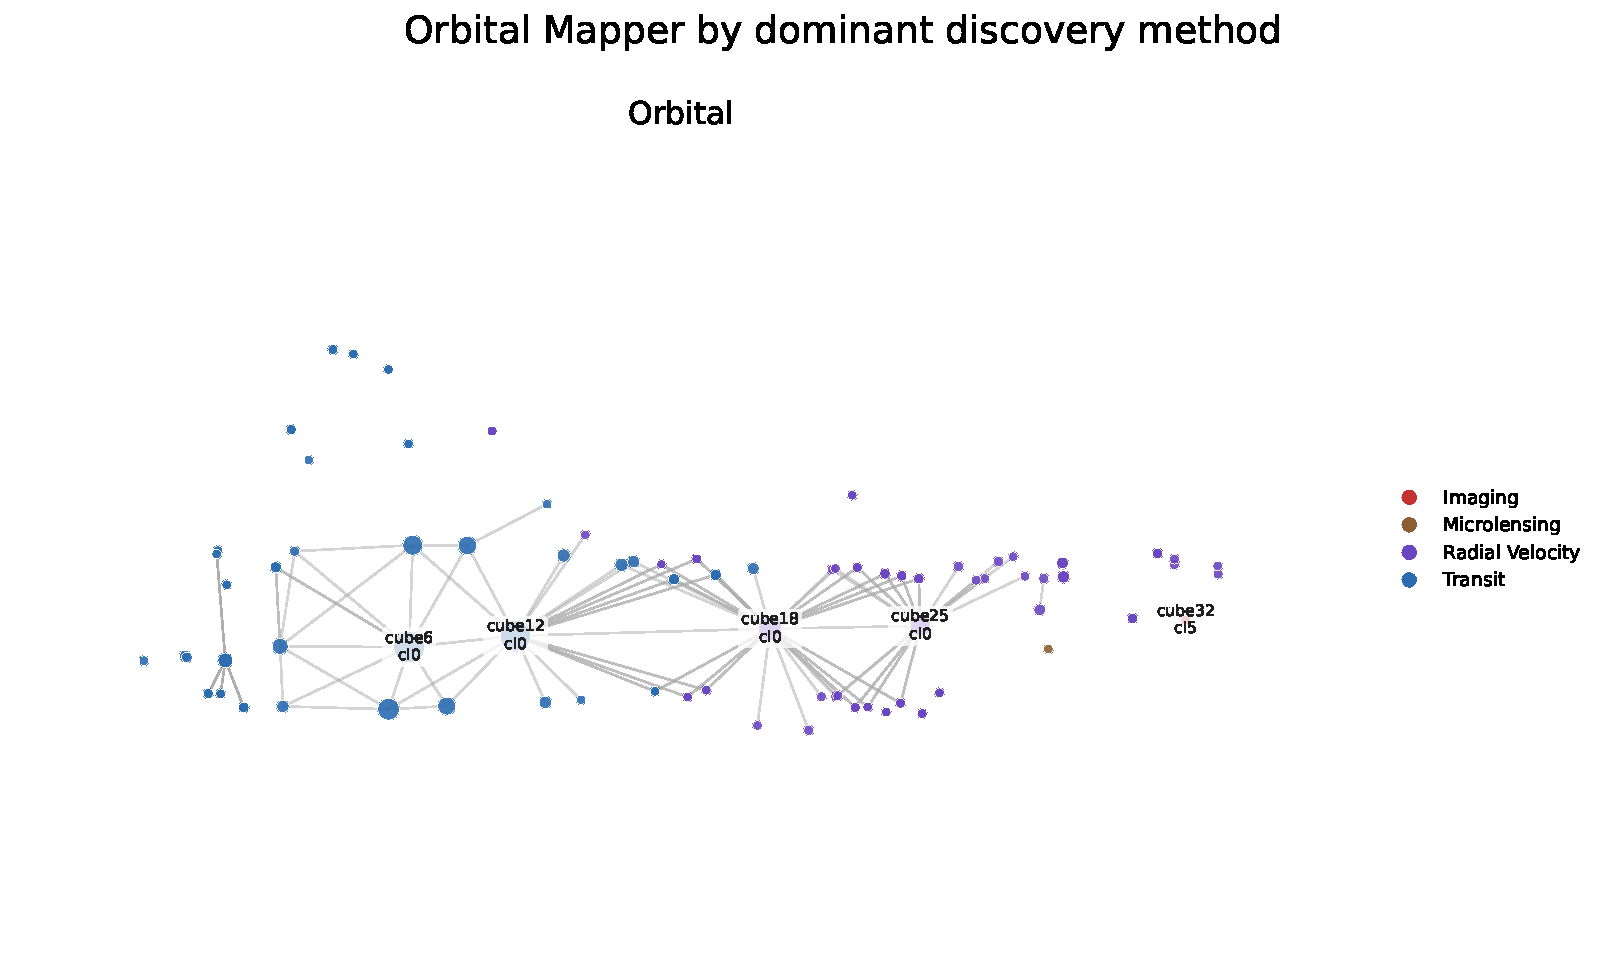
\includegraphics[width=0.78\linewidth]{figures/orbital_graph_discoverymethod.pdf}
\caption{Grafo orbital coloreado por método de descubrimiento dominante. La concentración de regiones por \texttt{discoverymethod} muestra que parte de la topología orbital está asociada con el proceso de detección.}
\label{fig:orbital_graph_discoverymethod}
\end{figure}

La Figura~\ref{fig:orbital_graph_discoverymethod} ayuda a interpretar por qué varias regiones orbitales terminan como \texttt{mixed}. Si ciertas zonas del grafo están dominadas por \texttt{Transit}, \texttt{Radial Velocity} o \texttt{Imaging}, entonces la estructura observada puede reflejar tanto arquitectura orbital como selección observacional. Esto no invalida el grafo orbital, pero sí impide interpretarlo como una señal orbital pura.

\begin{figure}[H]
\centering
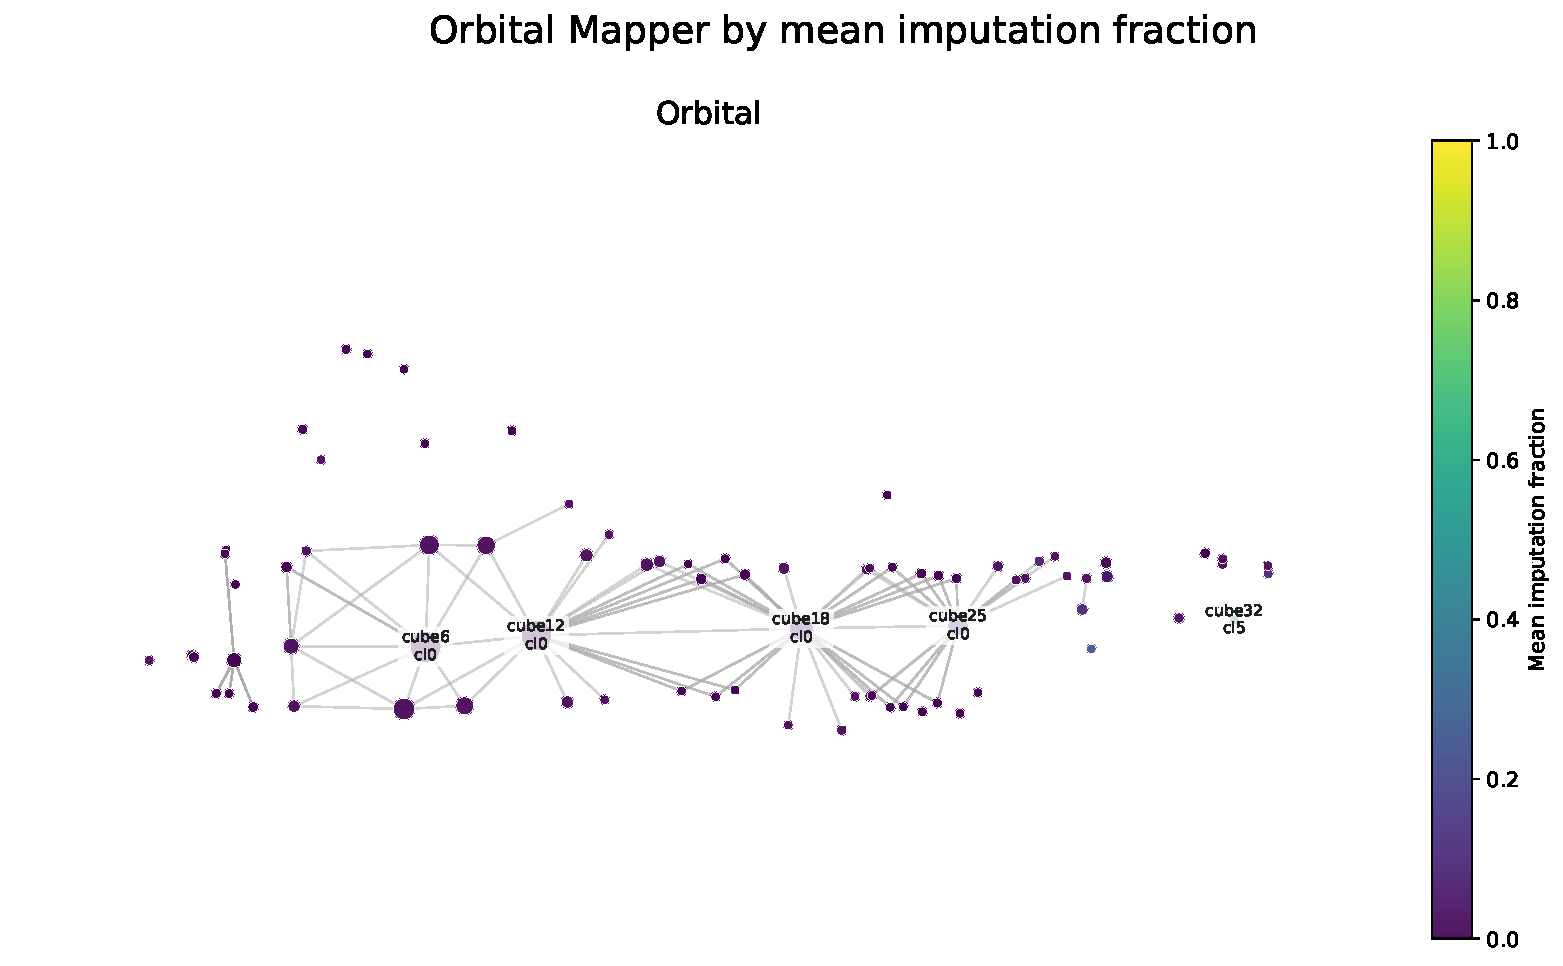
\includegraphics[width=0.78\linewidth]{figures/orbital_graph_imputation.pdf}
\caption{Grafo orbital coloreado por fracción de imputación. La baja imputación general del espacio orbital refuerza su valor como candidato de inspección, aunque la auditoría observacional obliga a una lectura mixta.}
\label{fig:orbital_graph_imputation}
\end{figure}

La Figura~\ref{fig:orbital_graph_imputation} muestra el otro lado de la interpretación. A diferencia del espacio térmico, el grafo orbital no está fuertemente sostenido por imputación. Por eso sigue siendo el resultado más informativo del proyecto. La tensión principal no es imputación, sino sesgo observacional: el grafo orbital es confiable en términos de datos, pero no independiente del proceso de descubrimiento.

\subsection*{Lectura de regiones \texttt{physical}}

Las regiones \texttt{physical} son las más defendibles para inspección científica posterior. En general, una región entra en esta categoría cuando muestra coherencia física u orbital, baja imputación y baja señal de enriquecimiento observacional. Estas regiones pueden corresponder a nodos con pureza de clase física relativamente alta, gradientes masa-radio coherentes o estructura orbital interpretable sin dominancia fuerte de un método de descubrimiento.

El número de regiones \texttt{physical} es bajo: 10 nodos. Esta escasez es importante. No significa que el catálogo no contenga señal astrofísica, sino que la evidencia limpia, bajo los criterios usados aquí, aparece en un subconjunto pequeño de regiones. En términos metodológicos, estas regiones son las mejores candidatas para inspección detallada, visualización individual y comparación con literatura astrofísica.

\subsection*{Lectura de regiones \texttt{observational}}

Las regiones \texttt{observational} aparecen cuando la evidencia está dominada por el proceso de descubrimiento. Esto puede ocurrir cuando una región tiene alta pureza por \texttt{discoverymethod}, baja entropía, enriquecimiento significativo bajo permutación, dominancia de una facilidad de descubrimiento o concentración temporal estrecha.

En los resultados finales, solo 1 nodo fue clasificado como \texttt{observational}, pero 4 componentes quedaron en esta categoría. Esto sugiere que las estructuras puramente observacionales son menos frecuentes que las mixtas, pero existen. Estas regiones no deben descartarse: también son científicamente informativas porque muestran cómo el catálogo está estructurado por la historia de observación. Sin embargo, no deben presentarse como evidencia física directa.

\subsection*{Lectura de regiones \texttt{mixed}}

La categoría \texttt{mixed} es la más importante para la interpretación global del proyecto. Una región \texttt{mixed} tiene algún patrón físico, orbital o térmico, pero también muestra señal observacional relevante. Esta categoría captura el comportamiento esperado en datos reales de exoplanetas: el catálogo no es una muestra uniforme de la población planetaria, sino el resultado de múltiples métodos, misiones, instrumentos y criterios de detección.

La abundancia de regiones \texttt{mixed} no significa que el análisis falló. Al contrario, muestra que Mapper está capturando estructuras que existen en el catálogo, pero que esas estructuras no pueden atribuirse de forma exclusiva a física planetaria. En particular, el grafo orbital cae en esta lectura: sigue siendo informativo por su complejidad y baja imputación, pero la asociación con \texttt{discoverymethod} obliga a interpretar muchas de sus regiones como mezcla de señal orbital y sesgo observacional.

\subsection*{Lectura de regiones \texttt{weak}}

Las regiones \texttt{weak} son aquellas donde la evidencia disponible no permite una interpretación fuerte. Esto puede deberse a alta imputación, tamaño pequeño del nodo o componente, evidencia física insuficiente, conflicto entre métricas o dependencia de variables menos confiables. Una región \texttt{weak} no significa que no exista estructura; significa que esa estructura no tiene soporte suficiente para sostener una conclusión astrofísica clara.

El número de nodos \texttt{weak} es alto: 245. Esto refuerza una de las lecciones metodológicas del proyecto. Mapper puede producir muchas regiones, pero no todas son igualmente interpretables. La síntesis final funciona precisamente como un filtro: evita que cada nodo del grafo sea tratado como una población significativa y prioriza únicamente aquellas regiones con mejor soporte.

\subsection*{Conclusión de la síntesis}

La síntesis final muestra que Mapper es útil para priorizar regiones de inspección, pero no para declarar una taxonomía final de exoplanetas. El predominio de regiones \texttt{mixed} y \texttt{weak} indica que la estructura observada está atravesada por sesgo observacional, imputación y decisiones metodológicas. Aun así, la presencia de regiones \texttt{physical} demuestra que sí existen candidatos con evidencia más limpia para análisis posterior.

El resultado principal de esta sección no es que Mapper descubra clases planetarias definitivas, sino que permite construir un mapa de evidencia. Bajo esta lectura, las regiones no se interpretan por su apariencia visual solamente, sino por la combinación de métricas que las sostienen. Esta es la contribución metodológica central del proyecto: separar estructura observada de interpretación astrofísica fuerte, y distinguir entre regiones físicas, observacionales, mixtas y débiles.
\section{Limitaciones}
Este analisis tiene limitaciones importantes. Primero, Mapper es exploratorio: resume una matriz procesada e imputada, pero no entrega la topologia real de los exoplanetas. Segundo, la cubierta reconciliada esta fija en 10 cubos y 0.35 de traslape; no se debe presentar como busqueda completa de hiperparametros. Tercero, \texttt{pl\_dens} puede estar derivada de masa y radio, por lo que no es evidencia independiente cuando se analiza junto con esas variables.

La prueba de permutacion de \texttt{discoverymethod} mide asociacion entre regiones Mapper y metadata observacional. No prueba causalidad. Una region enriquecida por metodo de descubrimiento puede corresponder a un sesgo instrumental, a una poblacion fisica que se descubre preferentemente por cierto metodo, o a una mezcla de ambas. Por eso el reporte usa categorias de evidencia y evita afirmar una clasificacion final de planetas.

\section{Conclusion}
La evidencia sugiere que los grafos Mapper seleccionados son utiles para priorizar regiones de inspeccion, siempre que se separen cuatro capas: senal fisica u orbital, sesgo observacional, dependencia de imputacion y sensibilidad al lens. El grafo orbital \texttt{orbital\_pca2\_cubes10\_overlap0p35} es un candidato importante por su complejidad y baja imputacion, pero la auditoria de sesgo muestra asociacion fuerte con \texttt{discoverymethod}; por tanto, debe interpretarse como evidencia mixta, no como estructura fisica pura.

La complejidad termica es especialmente cautelosa por su alta imputacion. La densidad funciona como control metodologico porque muchos valores de \texttt{pl\_dens} son derivados de masa y radio. La conclusion principal no es una taxonomia final, sino una clasificacion reproducible de regiones: algunas fisicamente interpretables, algunas observacionalmente sospechosas, muchas mixtas y otras debiles. Este resultado establece una base medible para una siguiente etapa de validacion, sin sobreafirmar la topologia real del catalogo.

\FloatBarrier
\clearpage
\begin{landscape}
\section*{Tablas complementarias}
\begin{table}[H]
\centering
\scriptsize
\caption{Sensibilidad por lens usando todos los artefactos existentes.}
\label{tab:lens_sensitivity}
\begin{adjustbox}{max width=\linewidth}
\begin{tabular}{llrrrr}
\toprule
feature\_space & lens & n\_nodes & n\_edges & beta\_1 & mean\_node\_imputation \\
\midrule
joint & density & 117 & 260 & 153 & 0.106 \\
joint & domain & 64 & 116 & 59 & 0.121 \\
joint & pca2 & 56 & 126 & 77 & 0.152 \\
joint\_no\_density & density & 109 & 233 & 134 & 0.142 \\
joint\_no\_density & domain & 9 & 0 & 0 & 0.212 \\
joint\_no\_density & pca2 & 62 & 134 & 81 & 0.176 \\
orb\_thermal & density & 121 & 246 & 138 & 0.255 \\
orb\_thermal & domain & 56 & 82 & 38 & 0.254 \\
orb\_thermal & pca2 & 58 & 100 & 54 & 0.347 \\
orbital & density & 178 & 297 & 144 & 0.030 \\
orbital & domain & 77 & 94 & 42 & 0.034 \\
orbital & pca2 & 124 & 196 & 96 & 0.011 \\
phys\_density & density & 78 & 109 & 52 & 0.002 \\
phys\_density & domain & 80 & 132 & 68 & 0.010 \\
phys\_density & pca2 & 67 & 102 & 52 & 0.002 \\
phys\_min & density & 97 & 152 & 75 & 0.010 \\
phys\_min & domain & 76 & 125 & 64 & 0.010 \\
phys\_min & pca2 & 66 & 105 & 54 & 0.017 \\
thermal & density & 205 & 338 & 171 & 0.472 \\
thermal & domain & 95 & 105 & 48 & 0.527 \\
thermal & pca2 & 121 & 150 & 67 & 0.588 \\
\bottomrule
\end{tabular}
\end{adjustbox}

\end{table}

\end{landscape}
\end{document}
